\chapter{Технологическая часть}
\section{Выбор СУБД}
Одними из наиболее популярных СУБД являются:
\begin{itemize}
	\item PostgreSQL~\cite{postgresql};
	\item MySQL~\cite{mysql};
	\item Microsoft SQL Server~\cite{msqlserver};
	\item Oracle~\cite{oracle}.
	
\end{itemize}


Для сравнения перечисленных выше СУБД были выделены следующие критерии:
\begin{itemize}
	\item распространяется бесплатно;
	\item наличие документации;
	\item возможность реализации триггеров;
	\item возможность реализации пользовательских функций;
	\item возможность индексирования;
	\item возможность реализации ролевой модели;
	\item поддержка стандарта SQL.
\end{itemize}

В таблице~\ref{pop_dbms} приведено сравнение перечисленных ранее СУБД по выделенным критериям.

\newpage
\begin{table}[ht]
	\begin{center}
		\begin{threeparttable}
			\caption{\label{pop_dbms} Сравнение СУБД}
			\begin{tabular}{|p{4cm}|p{3cm}|p{2.2cm}|p{3cm}|p{2cm}|c|}
				\hline
				\textbf{Критерий сравнения} & \textbf{PostgreSQL} & \textbf{MySQL} & \textbf{Microsoft SQL Server} & \textbf{Oracle} \\ \hline
				Распространяется бесплатно & + & + & -- & --\\ \hline
				Наличие документации & + & + & + & +\\ \hline
				Возможность реализации триггеров & + & + & + & +\\ \hline
				Возможность реализации пользовательских функций & + & + & + & +\\ \hline
				
				Возможность индексирования & + & + & + & +\\ \hline
				Возможность реализации ролевой модели & + & +/-- (с 8.0) & + & +\\ \hline
				Поддержка стандарта SQL & + & +/--(частично) & + & +\\ \hline
			\end{tabular}
		\end{threeparttable}
	\end{center}
\end{table}

Для решения поставленной задачи в качестве СУБД будет использоваться PоstgreSQL, в силу бесплатного распространения, возможности индексирования, создания пользовательских функций и триггеров, а также реализации ролевой модели.


\section{Выбор средств реализации пользовательского интерфейса}


Для разработки интерфейса доступа к базе данных были выбраны язык программирования C\#~\cite{csharp} и платформа .NET~\cite{dotnet}, поскольку они предоставляют возможность \hfill использования \hfill бесплатных \hfill инструментов \hfill для \hfill создания \\ \mbox{веб-приложений} и  библиотеки (драйвера) Npgsql~\cite{npgsql} для работы с PostgreSQL.

В качестве среды разработки была выбрана Visual Studio 2022~\cite{vs}, потому что она является бесплатной и автоматизирует этапы сборки и отладки приложения.

\newpage 
\section{Реализация объектов базы данных}
\subsection{Создание таблиц}


На листингах~\ref{create_roles}--\ref{create_favcoffeeshops} представлено создание всех таблиц базы данных, а также реализация упомянутых ранее ограничений целостности.
\begin{center}
	\captionsetup{justification=raggedright,singlelinecheck=off}
	\begin{lstlisting}[label=create_roles,caption=Создание таблицы roles]
CREATE TABLE IF NOT EXISTS roles (
	id_role INT PRIMARY KEY,
	name VARCHAR(128) NOT NULL, 
	CHECK (name = 'ordinary_user' OR name = 'moderator' OR name = 'administrator' OR name='guest')
);
		\end{lstlisting}
\end{center}

\begin{center}
	\captionsetup{justification=raggedright,singlelinecheck=off}
	\begin{lstlisting}[label=create_users,caption=Создание таблицы users]
CREATE TABLE IF NOT EXISTS users (
	id_user UUID PRIMARY KEY DEFAULT gen_random_uuid(),
	id_role INT NOT NULL,
	login VARCHAR(128) NOT NULL UNIQUE,
	password VARCHAR(128) NOT NULL,
	birthdate DATE NOT NULL,
	CHECK (birthdate < CURRENT_DATE),
	email VARCHAR(256) NOT NULL
);
ALTER TABLE users ADD FOREIGN KEY(id_role) REFERENCES roles(id_role);
	\end{lstlisting}
\end{center}

\begin{center}
	\captionsetup{justification=raggedright,singlelinecheck=off}
	\begin{lstlisting}[label=create_drinks,caption=Создание таблицы drinks]
CREATE TABLE IF NOT EXISTS drinks(
	id_drink UUID PRIMARY KEY DEFAULT gen_random_uuid(),
	name VARCHAR(128) NOT NULL UNIQUE
);
	\end{lstlisting}
\end{center}

\begin{center}
	\captionsetup{justification=raggedright,singlelinecheck=off}
	\begin{lstlisting}[label=create_categories,caption=Создание таблицы categories]
CREATE TABLE IF NOT EXISTS categories(
	id_category UUID PRIMARY KEY DEFAULT gen_random_uuid(),
	name VARCHAR(128) NOT NULL UNIQUE
);
	\end{lstlisting}
\end{center}

\begin{center}
	\captionsetup{justification=raggedright,singlelinecheck=off}
	\begin{lstlisting}[label=create_favdrinks,caption=Создание таблицы favdrinks]
CREATE TABLE IF NOT EXISTS favdrinks(
	id_user UUID NOT NULL,
	id_drink UUID NOT NULL,
	PRIMARY KEY (id_user, id_drink)
);
ALTER TABLE favdrinks ADD FOREIGN KEY(id_drink) REFERENCES drinks(id_drink);
ALTER TABLE favdrinks ADD FOREIGN KEY(id_user) REFERENCES users(id_user);
	\end{lstlisting}
\end{center}

\begin{center}
	\captionsetup{justification=raggedright,singlelinecheck=off}
	\begin{lstlisting}[label=create_drinkscategory,caption=Создание таблицы drinkscategory]
CREATE TABLE IF NOT EXISTS drinkscategory(
	id_drink UUID NOT NULL,
	id_category UUID NOT NULL,
	PRIMARY KEY (id_drink, id_category)
);
ALTER TABLE drinkscategory ADD FOREIGN KEY(id_drink) REFERENCES drinks(id_drink);
ALTER TABLE drinkscategory ADD FOREIGN KEY(id_category) REFERENCES categories(id_category);
	\end{lstlisting}
\end{center}


\begin{center}
	\captionsetup{justification=raggedright,singlelinecheck=off}
	\begin{lstlisting}[label=create_companies,caption=Создание таблицы companies]
CREATE TABLE IF NOT EXISTS companies(
	id_company UUID PRIMARY KEY DEFAULT gen_random_uuid(),
	name VARCHAR(128) NOT NULL,
	website VARCHAR (256),
	amountcoffeeshops INT NOT NULL DEFAULT 0,
	CHECK (amountcoffeeshops >= 0)
);
	\end{lstlisting}
\end{center}

\begin{center}
	\captionsetup{justification=raggedright,singlelinecheck=off}
	\begin{lstlisting}[label=create_lp,caption=Создание таблицы loyaltyprograms]
CREATE TABLE IF NOT EXISTS loyaltyprograms(
	id_lp UUID PRIMARY KEY DEFAULT gen_random_uuid(),
	id_company UUID NOT NULL,
	type TEXT,  
	description TEXT 
);  
ALTER TABLE loyaltyprograms ADD FOREIGN KEY(id_company) REFERENCES companies(id_company);
	\end{lstlisting}
\end{center}

\begin{center}
	\captionsetup{justification=raggedright,singlelinecheck=off}
	\begin{lstlisting}[label=create_menu,caption=Создание таблицы menu]
CREATE TABLE IF NOT EXISTS menu(
	id_menu UUID PRIMARY KEY DEFAULT gen_random_uuid(),
	id_drink UUID NOT NULL,
	id_company UUID NOT NULL,
	size INT NOT NULL,
	price NUMERIC(10,2) NOT NULL CHECK (price >= 0)
);
ALTER TABLE menu ADD FOREIGN KEY(id_drink) REFERENCES drinks(id_drink);
ALTER TABLE menu ADD FOREIGN KEY(id_company) REFERENCES companies(id_company);
	\end{lstlisting}
\end{center}

\begin{center}
	\captionsetup{justification=raggedright,singlelinecheck=off}
	\begin{lstlisting}[label=create_coffeeshops,caption=Создание таблицы coffeeshops]
CREATE TABLE IF NOT EXISTS coffeeshops(
	id_coffeeshop UUID PRIMARY KEY DEFAULT gen_random_uuid(),
	id_company UUID NOT NULL,
	address VARCHAR(256) NOT NULL,
	workinghours VARCHAR(64) NOT NULL
);
ALTER TABLE coffeeshops ADD FOREIGN KEY(id_company) REFERENCES companies(id_company);
	\end{lstlisting}
\end{center}

\begin{center}
	\captionsetup{justification=raggedright,singlelinecheck=off}
	\begin{lstlisting}[label=create_favcoffeeshops,caption=Создание таблицы favcoffeeshops]
CREATE TABLE IF NOT EXISTS favcoffeeshops(
	id_user UUID NOT NULL,
	id_coffeeshop UUID NOT NULL,
	PRIMARY KEY (id_user, id_coffeeshop)
);
ALTER TABLE favcoffeeshops ADD FOREIGN KEY(id_coffeeshop) REFERENCES coffeeshops(id_coffeeshop);
ALTER TABLE favcoffeeshops ADD FOREIGN KEY(id_user) REFERENCES users(id_user);
	\end{lstlisting}
\end{center}

\subsection{Создание триггеров}
На листингах~\ref{create_trigger_drink}--\ref{create_trigger_decr} представлено создание описанных в конструкторской части триггеров. Для каждого из триггеров сначала создается функция, которая будет выполнена автоматически при наступлении соответствующего события.
\begin{center}
	\captionsetup{justification=raggedright,singlelinecheck=off}
	\begin{lstlisting}[label=create_trigger_drink,caption={Создание триггера, удаляещего из таблиц menu, favdrinks и drinkscategory все записи, связанные с удаляемым из таблицы drinks напитком}]
CREATE OR REPLACE FUNCTION delete_drinks_records()
RETURNS TRIGGER AS $$
BEGIN
	DELETE FROM menu WHERE id_drink = OLD.id_drink;
	DELETE FROM favdrinks WHERE id_drink = OLD.id_drink;
	DELETE FROM drinkscategory WHERE id_drink = OLD.id_drink;
	RETURN OLD;
END;
$$ LANGUAGE plpgsql;

CREATE TRIGGER before_delete_drink BEFORE DELETE ON drinks FOR EACH ROW EXECUTE FUNCTION delete_drinks_records();
	\end{lstlisting}
\end{center}

\begin{center}
	\captionsetup{justification=raggedright,singlelinecheck=off}
	\begin{lstlisting}[label=create_trigger_cshop,caption={Создание триггера, удаляещего из таблицы favcoffeeshops все записи, связанные с удаляемой из таблицы coffeeshops кофейней}]
CREATE OR REPLACE FUNCTION delete_cshop_records()
RETURNS TRIGGER AS $$
BEGIN
	DELETE FROM favcoffeeshops WHERE id_coffeeshop = OLD.id_coffeeshop;
	RETURN OLD;
END;
$$ LANGUAGE plpgsql;

CREATE TRIGGER before_delete_coffeeshop BEFORE DELETE ON coffeeshops FOR EACH ROW EXECUTE FUNCTION delete_cshop_records();
	\end{lstlisting}
\end{center}

\begin{center}
	\captionsetup{justification=raggedright,singlelinecheck=off}
	\begin{lstlisting}[label=create_trigger_user,caption={Создание триггера, удаляещего из таблиц favcoffeeshops и favdrinks все записи, связанные с удаляемым из таблицы users пользователем}]
CREATE OR REPLACE FUNCTION delete_user_records()
RETURNS TRIGGER AS $$
BEGIN
	DELETE FROM favcoffeeshops WHERE id_user = OLD.id_user;
	DELETE FROM favdrinks WHERE id_user = OLD.id_user;
	RETURN OLD;
END;
$$ LANGUAGE plpgsql;

CREATE TRIGGER before_delete_user BEFORE DELETE ON user FOR EACH ROW EXECUTE FUNCTION delete_user_records();
	\end{lstlisting}
\end{center}

\begin{center}
	\captionsetup{justification=raggedright,singlelinecheck=off}
	\begin{lstlisting}[label=create_trigger_incr,caption={Создание триггера, инкрементирующего значение поля amountcoffeeshops таблицы companies}]
CREATE OR REPLACE FUNCTION increment_amount_coffeeshops()
RETURNS TRIGGER AS $$
BEGIN
	UPDATE companies
	SET amountcoffeeshops = amountcoffeeshops + 1
	WHERE id_company = NEW.id_company;
	RETURN NEW;
END;
$$ LANGUAGE plpgsql;

CREATE TRIGGER after_insert_coffeeshop AFTER INSERT ON coffeeshops FOR EACH ROW EXECUTE FUNCTION increment_amount_coffeeshops();
	\end{lstlisting}
\end{center}

\begin{center}
	\captionsetup{justification=raggedright,singlelinecheck=off}
	\begin{lstlisting}[label=create_trigger_decr,caption={Создание триггера, декрементирующего значение поля amountcoffeeshops таблицы companies}]
CREATE OR REPLACE FUNCTION decrement_amount_coffeeshops()
RETURNS TRIGGER AS $$
BEGIN
	UPDATE companies
	SET amountcoffeeshops = amountcoffeeshops - 1
	WHERE id_company = OLD.id_company;
	RETURN OLD;
END;
$$ LANGUAGE plpgsql;

CREATE TRIGGER after_delete_coffeeshop AFTER DELETE ON coffeeshops
FOR EACH ROW EXECUTE FUNCTION decrement_amount_coffeeshops();
	\end{lstlisting}
\end{center}

\newpage
\subsection{Создание функций}
На листинге~\ref{create_func_menu} представлено создание подставляемой табличной функции, которая по идентификатору напитка находит сети кофеен, в меню которых представлен данный напиток.


\begin{center}
	\captionsetup{justification=raggedright,singlelinecheck=off}
	\begin{lstlisting}[label=create_func_menu,caption={Создание функции, которая по идентификатору напитка находит сети кофеен, в меню которых представлен этот напиток}]
CREATE OR REPLACE FUNCTION companies_by_drink(drink_id uuid)
RETURNS TABLE ( id_company uuid, name VARCHAR(128), website VARCHAR(256), amountcoffeeshops INT
) 
AS $$
BEGIN
RETURN QUERY
	SELECT c.id_company, c.name, c.website, c.amountcoffeeshops
	FROM companies c
	WHERE  c.id_company in (select m.id_company from menu m where m.id_drink = drink_id);
END;
$$ LANGUAGE plpgsql;
	\end{lstlisting}
\end{center}

На листинге~\ref{create_proc} представлено создание хранимой процедуры, которая изменяет права доступа пользователей.
\begin{center}
	\captionsetup{justification=raggedright,singlelinecheck=off}
	\begin{lstlisting}[label=create_proc,caption={Создание хранимой процедуры, которая изменяет права доступа пользователей.}]
CREATE OR REPLACE PROCEDURE update_user_rights(user_id UUID, new_role_id INT)
LANGUAGE plpgsql
AS $$
BEGIN
	UPDATE users SET id_role = new_role_id WHERE id_user = user_id;
END;
$$;
	\end{lstlisting}
\end{center}

\newpage
\subsection{Создание ролевой модели}
На листинге~\ref{create_guest} представлено создание
роли гостя и выдача ему необходимых прав в соответствии с диаграммой прецедентов, представленной на рисунке~\ref{usecase_all}.
\begin{center}
	\captionsetup{justification=raggedright,singlelinecheck=off}
	\begin{lstlisting}[label=create_guest,caption={Создание роли гостя}]
CREATE ROLE guest WITH LOGIN PASSWORD 'guest2025';
GRANT SELECT, INSERT ON users TO guest;
GRANT SELECT ON roles TO guest;
	\end{lstlisting}
\end{center}

На листинге~\ref{create_user} представлено создание
роли обычного пользователя и выдача ему необходимых прав в соответствии с диаграммой прецедентов, представленной на рисунке~\ref{usecase_all}.
\begin{center}
	\captionsetup{justification=raggedright,singlelinecheck=off}
	\begin{lstlisting}[label=create_user,caption={Создание роли обычного пользователя}]
CREATE ROLE ordinary_user WITH LOGIN PASSWORD 'user2025';
GRANT SELECT, INSERT, DELETE, UPDATE ON users TO ordinary_user;
GRANT SELECT ON drinks TO ordinary_user ;
GRANT SELECT ON companies TO ordinary_user ;
GRANT SELECT ON coffeeshops TO ordinary_user ;
GRANT SELECT ON categories TO ordinary_user ;
GRANT SELECT ON drinkscategory TO ordinary_user ;
GRANT SELECT ON menu TO ordinary_user ;
GRANT SELECT ON loyaltyprograms TO ordinary_user ;
GRANT SELECT, INSERT, DELETE ON favdrinks TO ordinary_user ;
GRANT SELECT,INSERT, DELETE ON favcoffeeshops TO ordinary_user ;
GRANT SELECT ON roles TO ordinary_user ;
	\end{lstlisting}
\end{center}

На листинге~\ref{create_moder} представлено создание
роли модератора и выдача ему необходимых прав в соответствии с диаграммой прецедентов, представленной на рисунке~\ref{usecase_all}.

\newpage
\begin{center}
	\captionsetup{justification=raggedright,singlelinecheck=off}
	\begin{lstlisting}[label=create_moder,caption={Создание роли модератора}]
CREATE ROLE moderator WITH LOGIN PASSWORD 'moder2025';
GRANT SELECT, INSERT, DELETE, UPDATE ON users TO moderator;
GRANT SELECT, INSERT, DELETE ON drinks TO moderator ;
GRANT SELECT, UPDATE ON companies TO moderator;
GRANT SELECT, INSERT, DELETE ON coffeeshops TO moderator;
GRANT SELECT, INSERT ON categories TO moderator;
GRANT SELECT, INSERT, DELETE, update ON drinkscategory TO moderator;
GRANT SELECT,INSERT, DELETE ON menu TO moderator;
GRANT SELECT ON loyaltyprograms TO moderator;
GRANT SELECT, INSERT, DELETE ON favdrinks TO moderator;
GRANT SELECT, INSERT, DELETE ON favcoffeeshops TO moderator;
GRANT SELECT ON roles TO moderator;
	\end{lstlisting}
\end{center}

На листинге~\ref{create_admin} представлено создание
роли администратора и выдача ему необходимых прав в соответствии с диаграммой прецедентов, представленной на рисунке~\ref{usecase_all}.
\begin{center}
	\captionsetup{justification=raggedright,singlelinecheck=off}
	\begin{lstlisting}[label=create_admin,caption={Создание роли администратора}]
CREATE ROLE administrator WITH LOGIN PASSWORD 'admin2025';
GRANT SELECT,INSERT, DELETE ON drinks TO administrator;
GRANT SELECT, UPDATE ON companies TO administrator;
GRANT SELECT,INSERT, DELETE ON coffeeshops TO administrator;
GRANT SELECT, INSERT ON categories TO administrator;
GRANT SELECT, INSERT, DELETE, UPDATE ON drinkscategory TO administrator;
GRANT SELECT,INSERT, DELETE ON menu TO administrator;
GRANT SELECT ON loyaltyprograms TO administrator;
GRANT SELECT, INSERT, DELETE ON favdrinks TO administrator;
GRANT SELECT,INSERT, DELETE ON favcoffeeshops TO administrator;
GRANT SELECT ON roles TO administrator;
GRANT SELECT, INSERT, DELETE, UPDATE ON users TO administrator;
	\end{lstlisting}
\end{center}


\newpage
\section{Тестирование}
Корректность работы триггеров на удаление записей была проверена путем тестирования. В таблицах~\ref{test_trigger}--\ref{test_cshop_trigger} описаны тестовые случаи. Все тесты были успешно пройдены.


\begin{table}[ht]
	\begin{center}
		\begin{threeparttable}
			\caption{\label{test_trigger} Тесты для триггера, который удаляет из таблиц menu, favdrinks и drinkscategory все записи, связанные с удаляемым из таблицы drinks напитком.}
			\begin{tabular}{|p{6cm}|p{4.5cm}|p{4.5cm}|c|}
				\hline    
				\textbf{\makecell{Описание теста}} & \textbf{\makecell{Ожидаемый\\результат}} & \textbf{\makecell{Полученный\\результат}} \\ \hline
				\multicolumn{3}{|c|}{\textbf{Напиток присутствует в связанных таблицах}} \\ \hline
				Напиток присутствует во всех таблицах menu, favdrinks, drinkscategory & Удалены запись из drinks и все связанные записи из menu, favdrinks и drinkscategory & Удалены запись из drinks и все связанные записи из menu, favdrinks и drinkscategory  \\ \hline
				Напиток присутствует только в таблице menu &  Удалены запись из drinks и menu & Удалены запись из drinks и menu \\ \hline
				Напиток присутствует только в таблице drinkscategory & Удалена запись из drinks и удалены  и drinkcategory & Удалена запись из drinks и удалены  и drinkcategory \\ \hline
				Напиток присутствует только в таблице favdrinks & Удалена запись из drinks и удалены  и favdrinks &  Удалена запись из drinks и удалены  и favdrinks \\ \hline
				\multicolumn{3}{|c|}{\textbf{Напиток отсутствует в связанных таблицах}} \\ \hline
				Напиток отсутствует в таблицах menu, favdrinks, drinkscategory & Удалена только запись из drinks & Удалена только запись из drinks \\ \hline
				\multicolumn{3}{|c|}{\textbf{Некорректный drink\_id напитка}} \\ \hline
				Попытка удаления несуществующего в drinks напитка & Никаких изменений в БД & Никаких изменений в БД \\ \hline
				Удаление напитка с id\_drink=NULL & Никаких изменений в БД & Никаких изменений в БД \\ \hline

			\end{tabular}
		\end{threeparttable}
	\end{center}
\end{table}

\begin{table}[H]
	\begin{center}
		\begin{threeparttable}
			\caption{\label{test_user_trigger} Тесты для триггера, который удаляет из таблиц favcoffeeshops и favdrinks все записи, связанные с удаляемым из таблицы users пользователем}
			\begin{tabular}{|p{6cm}|p{4.5cm}|p{4.5cm}|}
				\hline    
			\textbf{\makecell{Описание теста}} & \textbf{\makecell{Ожидаемый\\результат}} & \textbf{\makecell{Полученный\\результат}} \\ \hline
				\multicolumn{3}{|c|}{\textbf{Пользователь присутствует в cвязанных таблицах}} \\ \hline
				Пользователь имеет записи в favcoffeeshops и favdrinks &  Удалены запись из users и все связанные  записи из favcoffeeshops и favdrinks & Удалены запись из users и все связанные записи из favcoffeeshops и favdrinks \\ \hline
				
				Пользователь имеет записи только в favcoffeeshops & Удалены записи из users и favcoffeeshops & Удалены записи из users и favcoffeeshops \\ \hline
				Пользователь имеет записи только в favdrinks & Удалены записи из users и favdrinks & Удалены записи из users и favdrinks \\ \hline
				\multicolumn{3}{|c|}{\textbf{Пользователь отсутствует в связанных таблицах}} \\ \hline
				Пользователь не имеет записей в favcoffeeshops и favdrinks & Удалена только запись из users & Удалена только запись из users \\ \hline
				\multicolumn{3}{|c|}{\textbf{Некорректный id\_user}} \\ \hline
				Попытка удаления несуществующего в users пользователя & Никаких изменений в БД & Никаких изменений в БД \\ \hline
				Удаление пользователя с id\_user=NULL & Никаких изменений в БД & Никаких изменений в БД \\ \hline
			\end{tabular}
		\end{threeparttable}
	\end{center}
\end{table}

\begin{table}[H]
	\begin{center}
		\begin{threeparttable}
			\caption{\label{test_cshop_trigger} Тесты для триггера, который удаляет из таблицы favcoffeeshops все записи, связанные с удаляемой из таблицы coffeeshops кофейней.}
			\begin{tabular}{|p{6cm}|p{4.5cm}|p{4.5cm}|c|}
				\hline    
				\textbf{\makecell{Описание теста}} & \textbf{\makecell{Ожидаемый\\результат}} & \textbf{\makecell{Полученный\\результат}}\\ \hline
				\multicolumn{3}{|c|}{\textbf{Кофейня присутствует в связанной таблице}} \\ \hline
				Кофейня присутствует в таблице favcoffeeshops & Удалены запись из coffeeshops и все связанные  записи из favcoffeeshops & Удалены запись из coffeeshops и все связанные  записи из favcoffeeshops \\ \hline
				\multicolumn{3}{|c|}{\textbf{Кофейня отсутствует в связанной таблице}} \\ \hline
				Кофейня отсутствует в таблице favcoffeeshops & Удалена только запись из coffeeshops & Удалена только запись из coffeeshops \\ \hline
				\multicolumn{3}{|c|}{\textbf{Некорректный id\_coffeeshop}} \\ \hline
				Попытка удаления несуществующей кофейни & Никаких изменений в БД & Никаких изменений в БД \\ \hline
				Удаление кофейни с id\_coffeeshop=NULL & Никаких изменений в БД & Никаких изменений в БД \\ \hline

			\end{tabular}
		\end{threeparttable}
	\end{center}
\end{table}



Корректность работы триггеров на обновление в таблице coffeeshops значения поля amountcoffeeshops была проверена путем тестирования. В таблицах~\ref{test_increment_trigger}--\ref{test_decrement_trigger} описаны тестовые случаи. Все тесты были успешно пройдены.
\begin{table}[H]
	\begin{center}
		\begin{threeparttable}
			\caption{\label{test_increment_trigger} Тесты для триггера, инкрементирующего значение поля amountcoffeeshops таблицы companies}
			\begin{tabular}{|p{6cm}|p{4.5cm}|p{4.5cm}|}
				\hline    
				\textbf{\makecell{Описание теста}} & \textbf{\makecell{Ожидаемый\\результат}} & \textbf{\makecell{Полученный\\результат}} \\ \hline

				Добавление новой кофейни, когда для соответствующей записи в companies amountcoffeeshops = 0  & amountcoffeeshops стал равным 1 & amountcoffeeshops стал равным 1 \\ \hline
				Добавление новой кофейни, когда для соответствующей записи в companies amountcoffeeshops = 5 & amountcoffeeshops стал равным 6 & amountcoffeeshops стал равным 6 \\ \hline

			\end{tabular}
		\end{threeparttable}
	\end{center}
\end{table}

\begin{table}[H]
	\begin{center}
		\begin{threeparttable}
			\caption{\label{test_decrement_trigger} Тесты для триггера, декрементирующего значение поля amountcoffeeshops таблицы companies}
			\begin{tabular}{|p{6cm}|p{4.5cm}|p{4.5cm}|}
				\hline    
				\textbf{\makecell{Описание теста}} & \textbf{\makecell{Ожидаемый\\результат}} & \textbf{\makecell{Полученный\\результат}}\\ \hline
				\multicolumn{3}{|c|}{\textbf{Успешное инкрементирование поля amountcoffeeshops}} \\ \hline
				Удаление кофейни, когда для соответствующей записи в companies amountcoffeeshops = 1  & amountcoffeeshops стал равным 0 & amountcoffeeshops стал равным 0 \\ \hline
				Удаление кофейни, когда для соответствующей записи в companies amountcoffeeshops = 4 & amountcoffeeshops стал равным 3 & amountcoffeeshops стал равным 3 \\ \hline

				\multicolumn{3}{|c|}{\textbf{Граничные случаи}} \\ \hline
				Удаление кофейни, когда для соответствующей записи в companies amountcoffeeshops = 0 & Значение amountcoffeeshops остаётся равным 0  & Значение amountcoffeeshops остаётся равным 0 \\ \hline

			\end{tabular}
		\end{threeparttable}
	\end{center}
\end{table}

Корректность работы функции companies\_by\_drink была проверена путем тестирования. В таблице~\ref{test_companies_by_drink} описаны тестовые случаи. Все тесты были успешно пройдены.

\begin{table}[H]
	\begin{center}
		\begin{threeparttable}
			\caption{\label{test_companies_by_drink} Тесты для функции companies\_by\_drink}
			\begin{tabular}{|p{6cm}|p{4.5cm}|p{4.5cm}|}
				\hline    
				\textbf{\makecell{Описание теста}} & \textbf{\makecell{Ожидаемый\\результат}} & \textbf{\makecell{Полученный\\результат}} \\ \hline
				\multicolumn{3}{|c|}{\textbf{Напиток принадлежит меню хотя бы одной компании}} \\ \hline
				Напиток есть в меню у одной компании & Возвращается 1 запись с данными компании &  Возвращается 1 запись с данными компании  \\ \hline
				

				Напиток есть в меню у 3 компаний & Возвращается 3 записи с данными компаний & Возвращается 3 записи с данными компаний \\ \hline
				\multicolumn{3}{|c|}{\textbf{Напиток не принадлежит ни одной компании}} \\ \hline
				Напиток существует в drinks, но отсутствует в таблице menu & Возвращается пустой результат (0 записей) & Возвращается пустой результат (0 записей) \\ \hline
				\multicolumn{3}{|c|}{\textbf{Функция вызывна для некорректного id\_drink}} \\ \hline
				Передан несуществующий drink\_id & Возвращается пустой результат (0 записей) & Возвращается пустой результат (0 записей)  \\ \hline
				Передан NULL в качестве drink\_id & Возвращается пустой результат (0 записей) & Возвращается пустой результат (0 записей) \\ \hline
			
			\end{tabular}
		\end{threeparttable}
	\end{center}
\end{table}

Корректность работы процедуры update\_user\_rights, изменяющей права доступа пользователя, была проверена путем тестирования. В таблице~\ref{test_update_user_rights} описаны тестовые случаи. Все тесты были успешно пройдены.

\begin{table}[H]
	\begin{center}
		\begin{threeparttable}
			\caption{\label{test_update_user_rights} Тесты для процедуры update\_user\_rights}
			\begin{tabular}{|p{6cm}|p{4.5cm}|p{4.5cm}|}
				\hline    
				\textbf{\makecell{Описание теста}} & \textbf{\makecell{Ожидаемый\\результат}} & \textbf{\makecell{Полученный\\результат}}\\ \hline
				\multicolumn{3}{|c|}{\textbf{В процедуру переданы корректные параметры}} \\ \hline
				Обновление роли пользователя с id\_user, сущ. в users, на new\_role\_id, сущ. в roles & id\_role изменён на new\_role\_id& id\_role изменён на new\_role\_id \\ \hline
				Обновление роли пользователя с id\_user, сущ. в users, на значение new\_role\_id  равное текущему id\_role& id\_role остался прежним & id\_role остался прежним \\ \hline
				
				\multicolumn{3}{|c|}{\textbf{В процедуру переданы некорректные параметры}} \\ \hline
				Передан несуществующий user\_id & 0 строк обновлено & 0 строк обновлено \\ \hline
				Передан несуществующий new\_role\_id & Ошибка внешнего ключа & Ошибка внешнего ключа \\ \hline

			\end{tabular}
		\end{threeparttable}
	\end{center}
\end{table}


\section{Интерфейс приложения}
Интерфейс веб-приложения разделен на страницы, каждая из которых предоставляет пользователю некоторые опции. На рисунках~\ref{login}--\ref{users} продемонстрирован интерфейс разработанного приложения.

\begin{figure}[H]
	\centering
	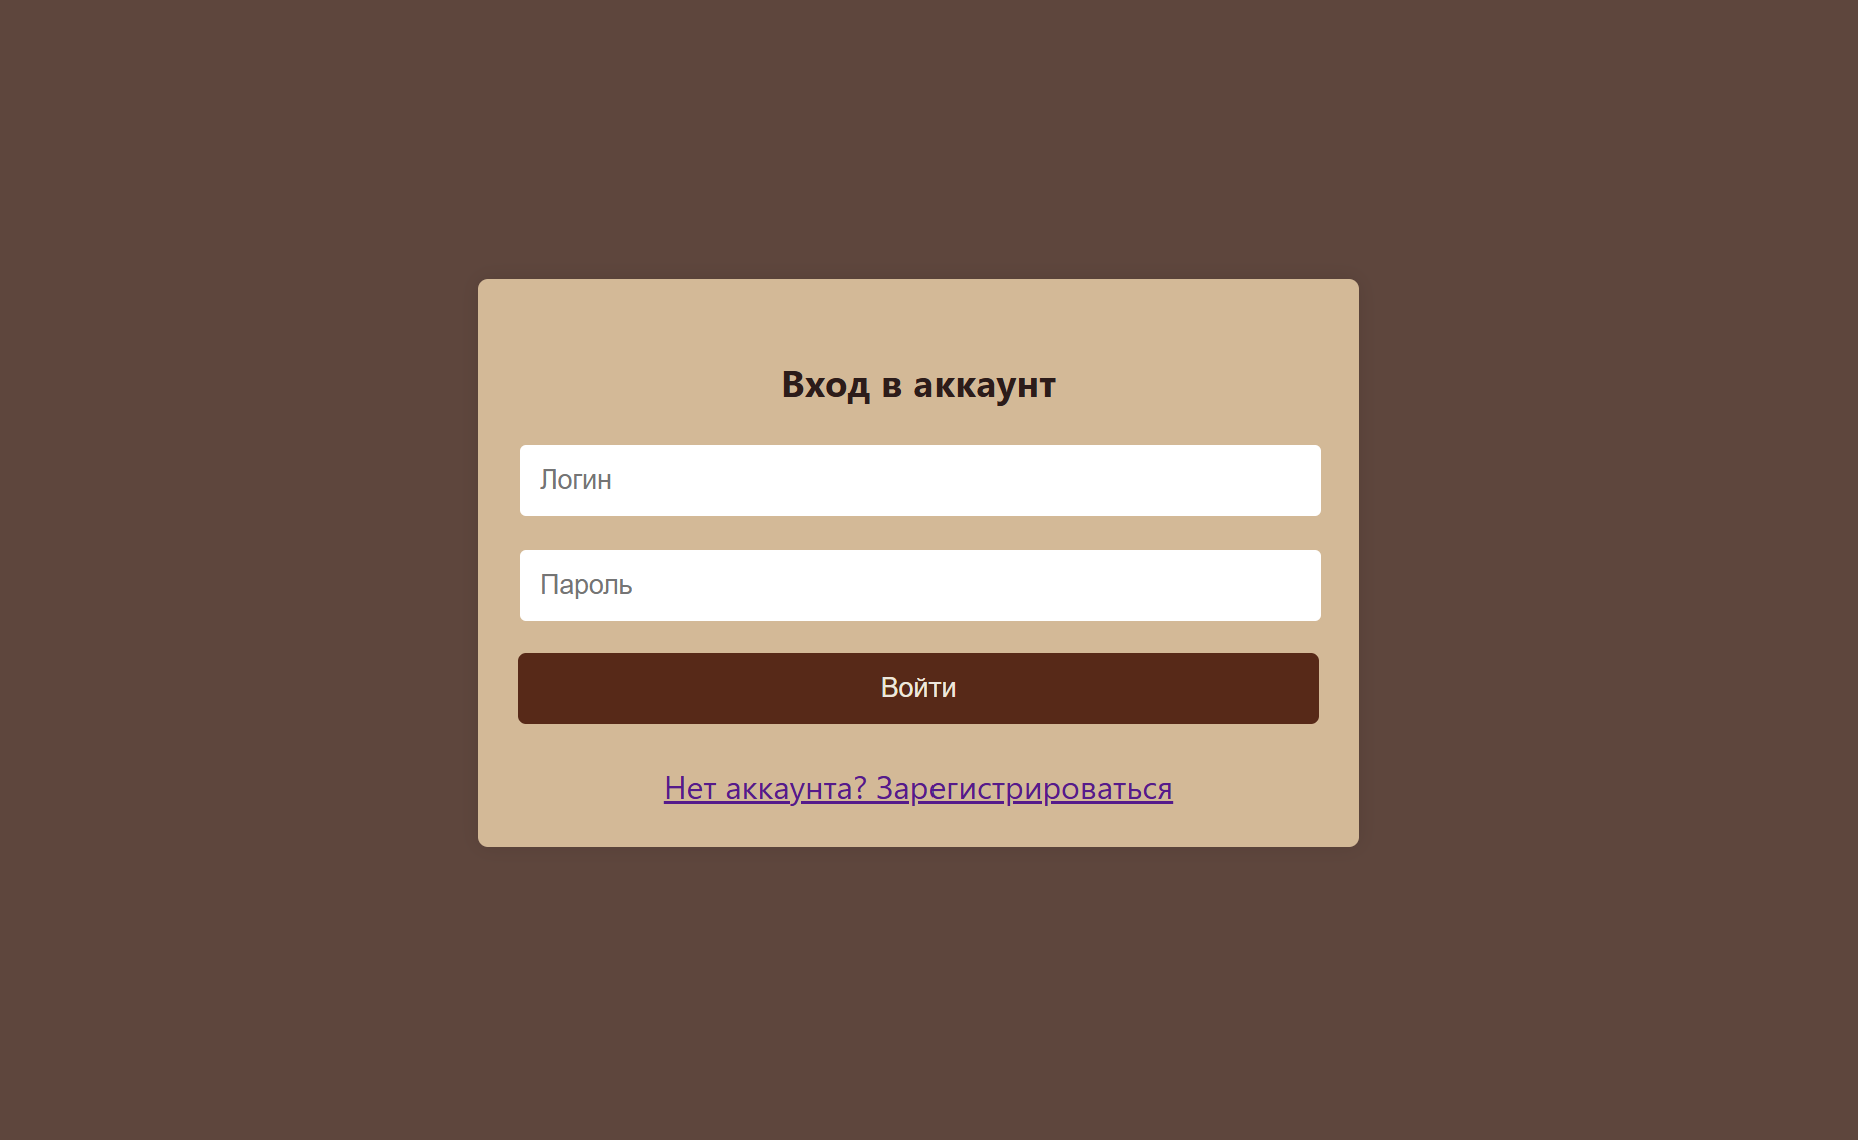
\includegraphics[width=1\linewidth]{img/interface/login.png}
	\caption{Страница авторизации}
	\label{login}
\end{figure}

\begin{figure}[H]
	\centering
	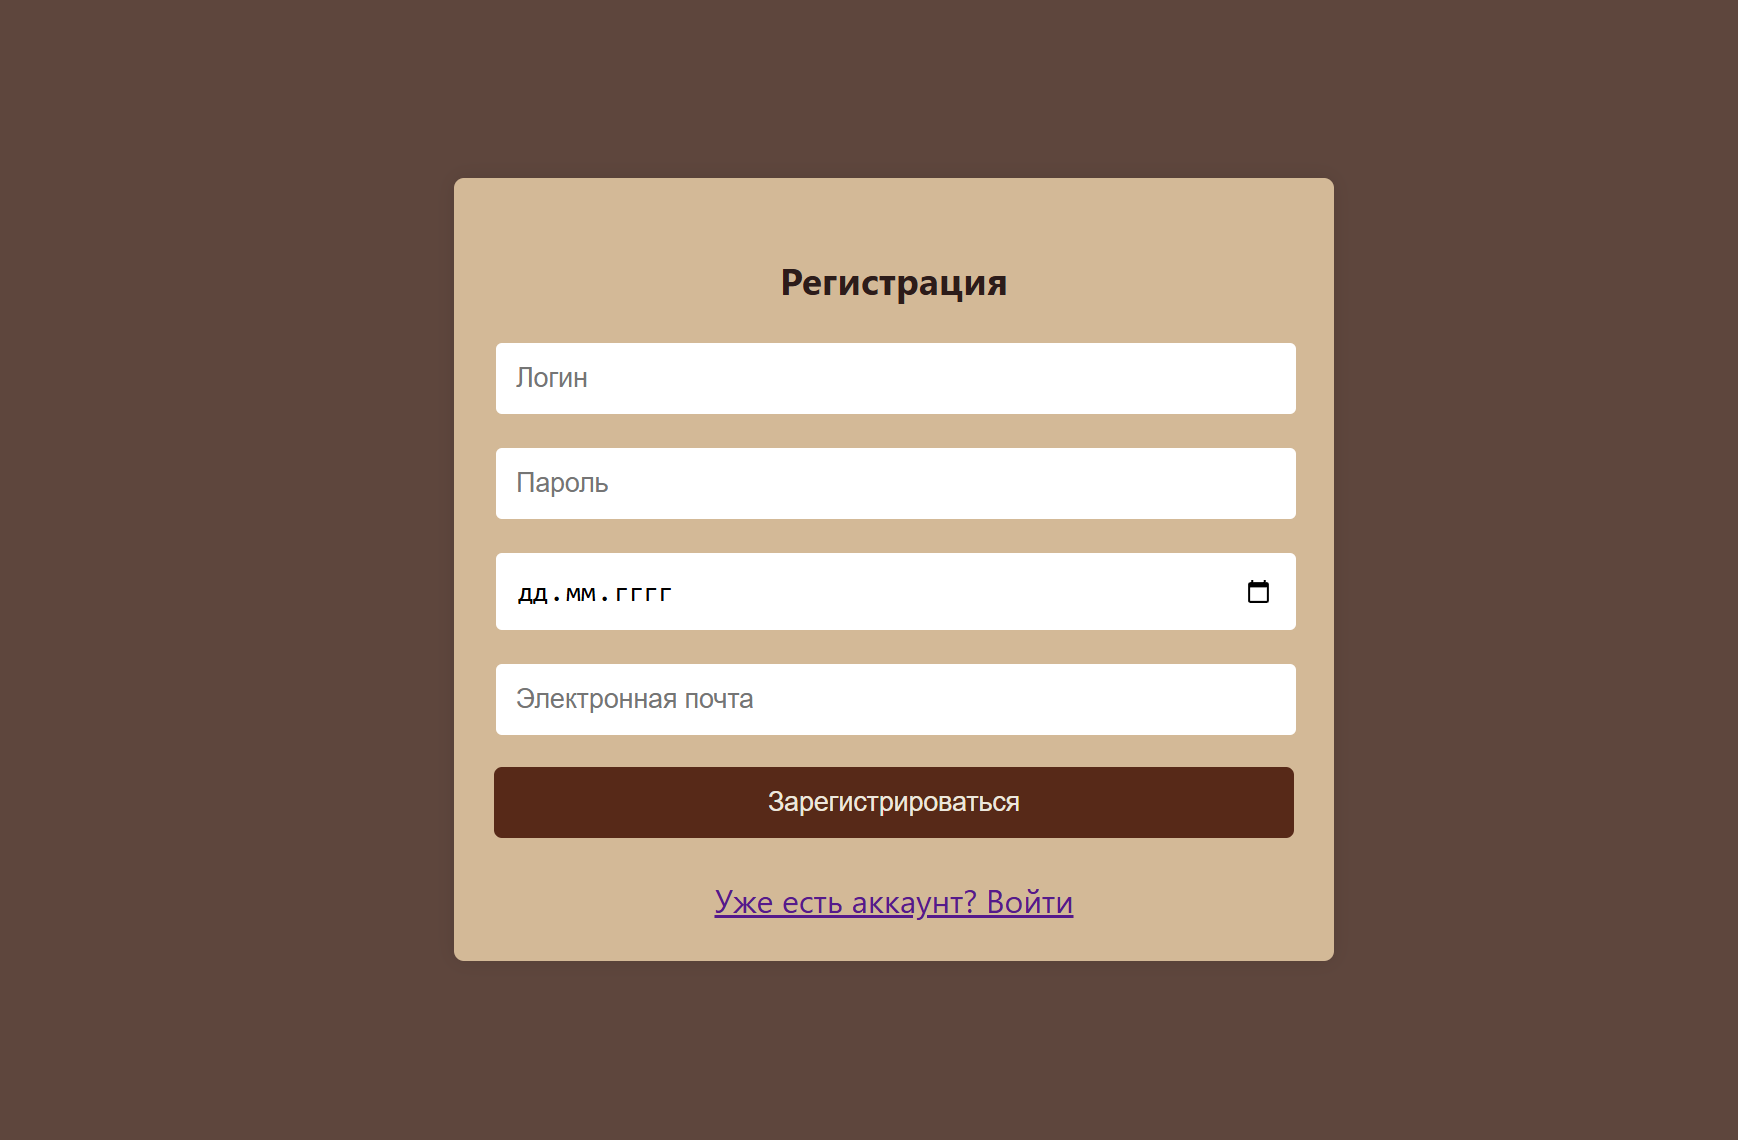
\includegraphics[width=1\linewidth]{img/interface/register.png}
	\caption{Страница регистрации}
	\label{register}
\end{figure}

\begin{figure}[H]
	\centering
	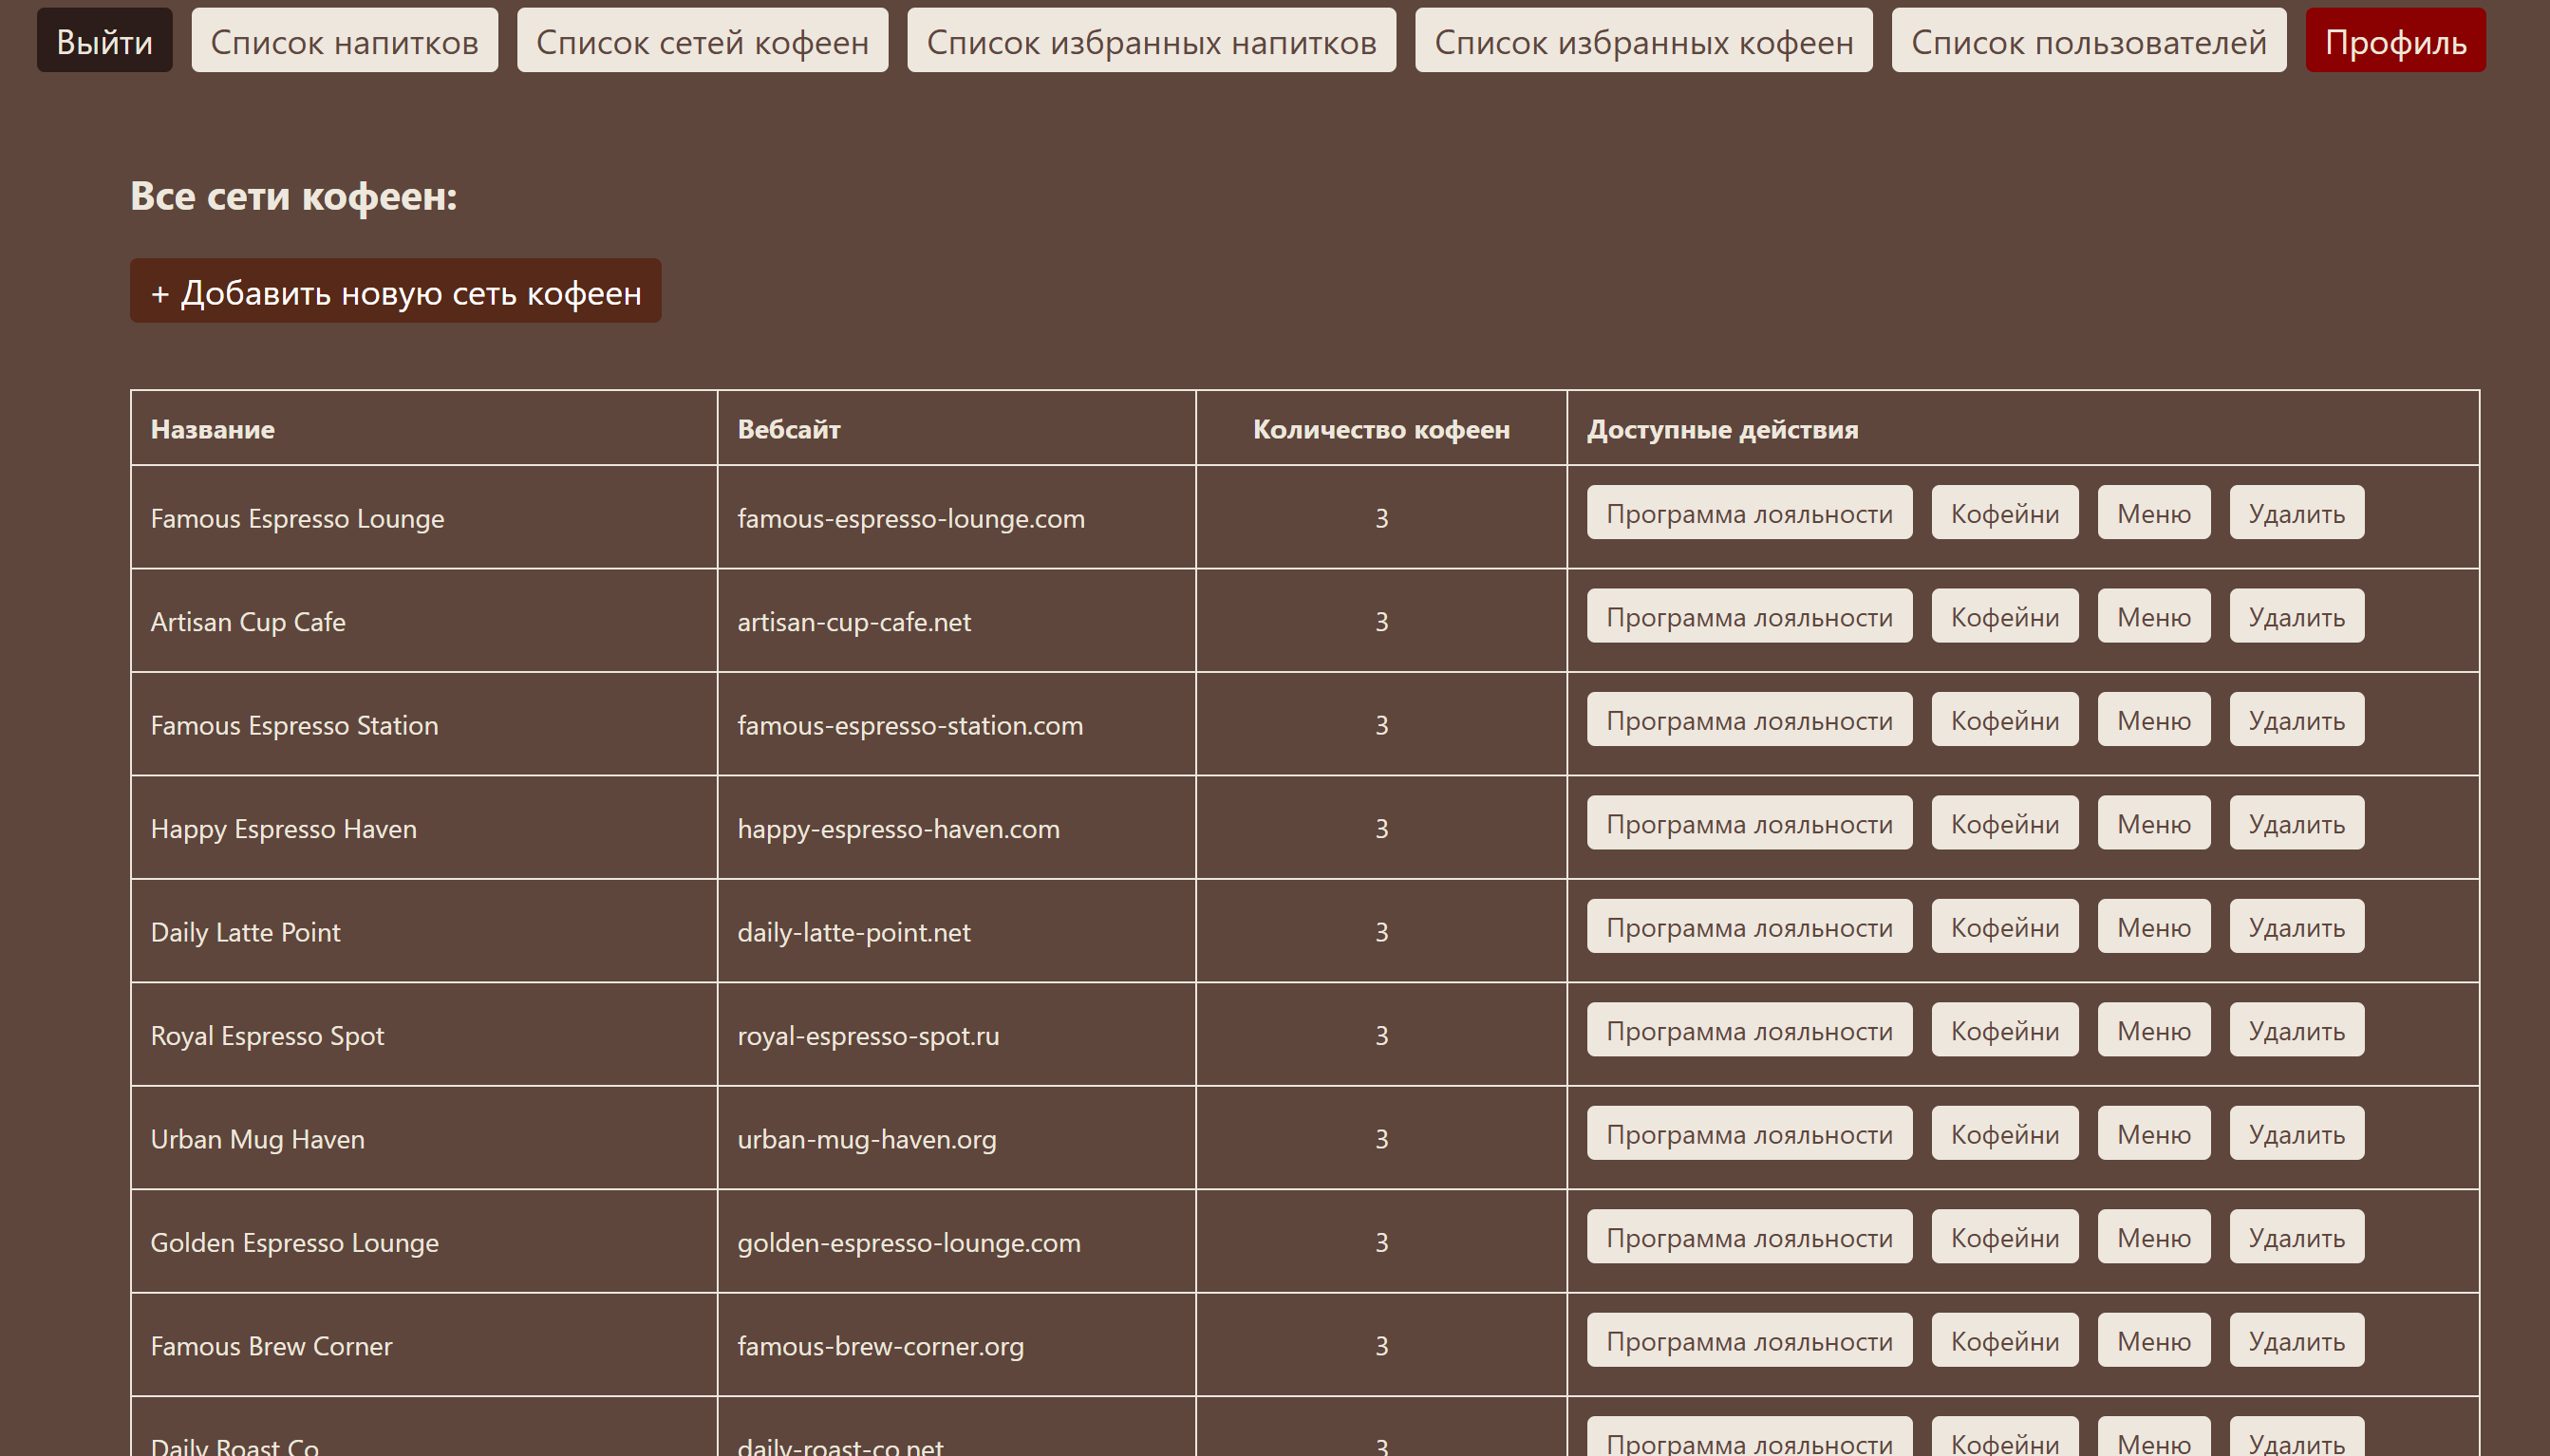
\includegraphics[width=1\linewidth]{img/interface/getallcompanies_admin.png}
	\caption{Страница с информацией о сетях кофеен (для обычных пользователей кнопки добавления и удаления сетей кофеен недоступны)}
	\label{getallcompanies}
\end{figure}

\begin{figure}[H]
	\centering
	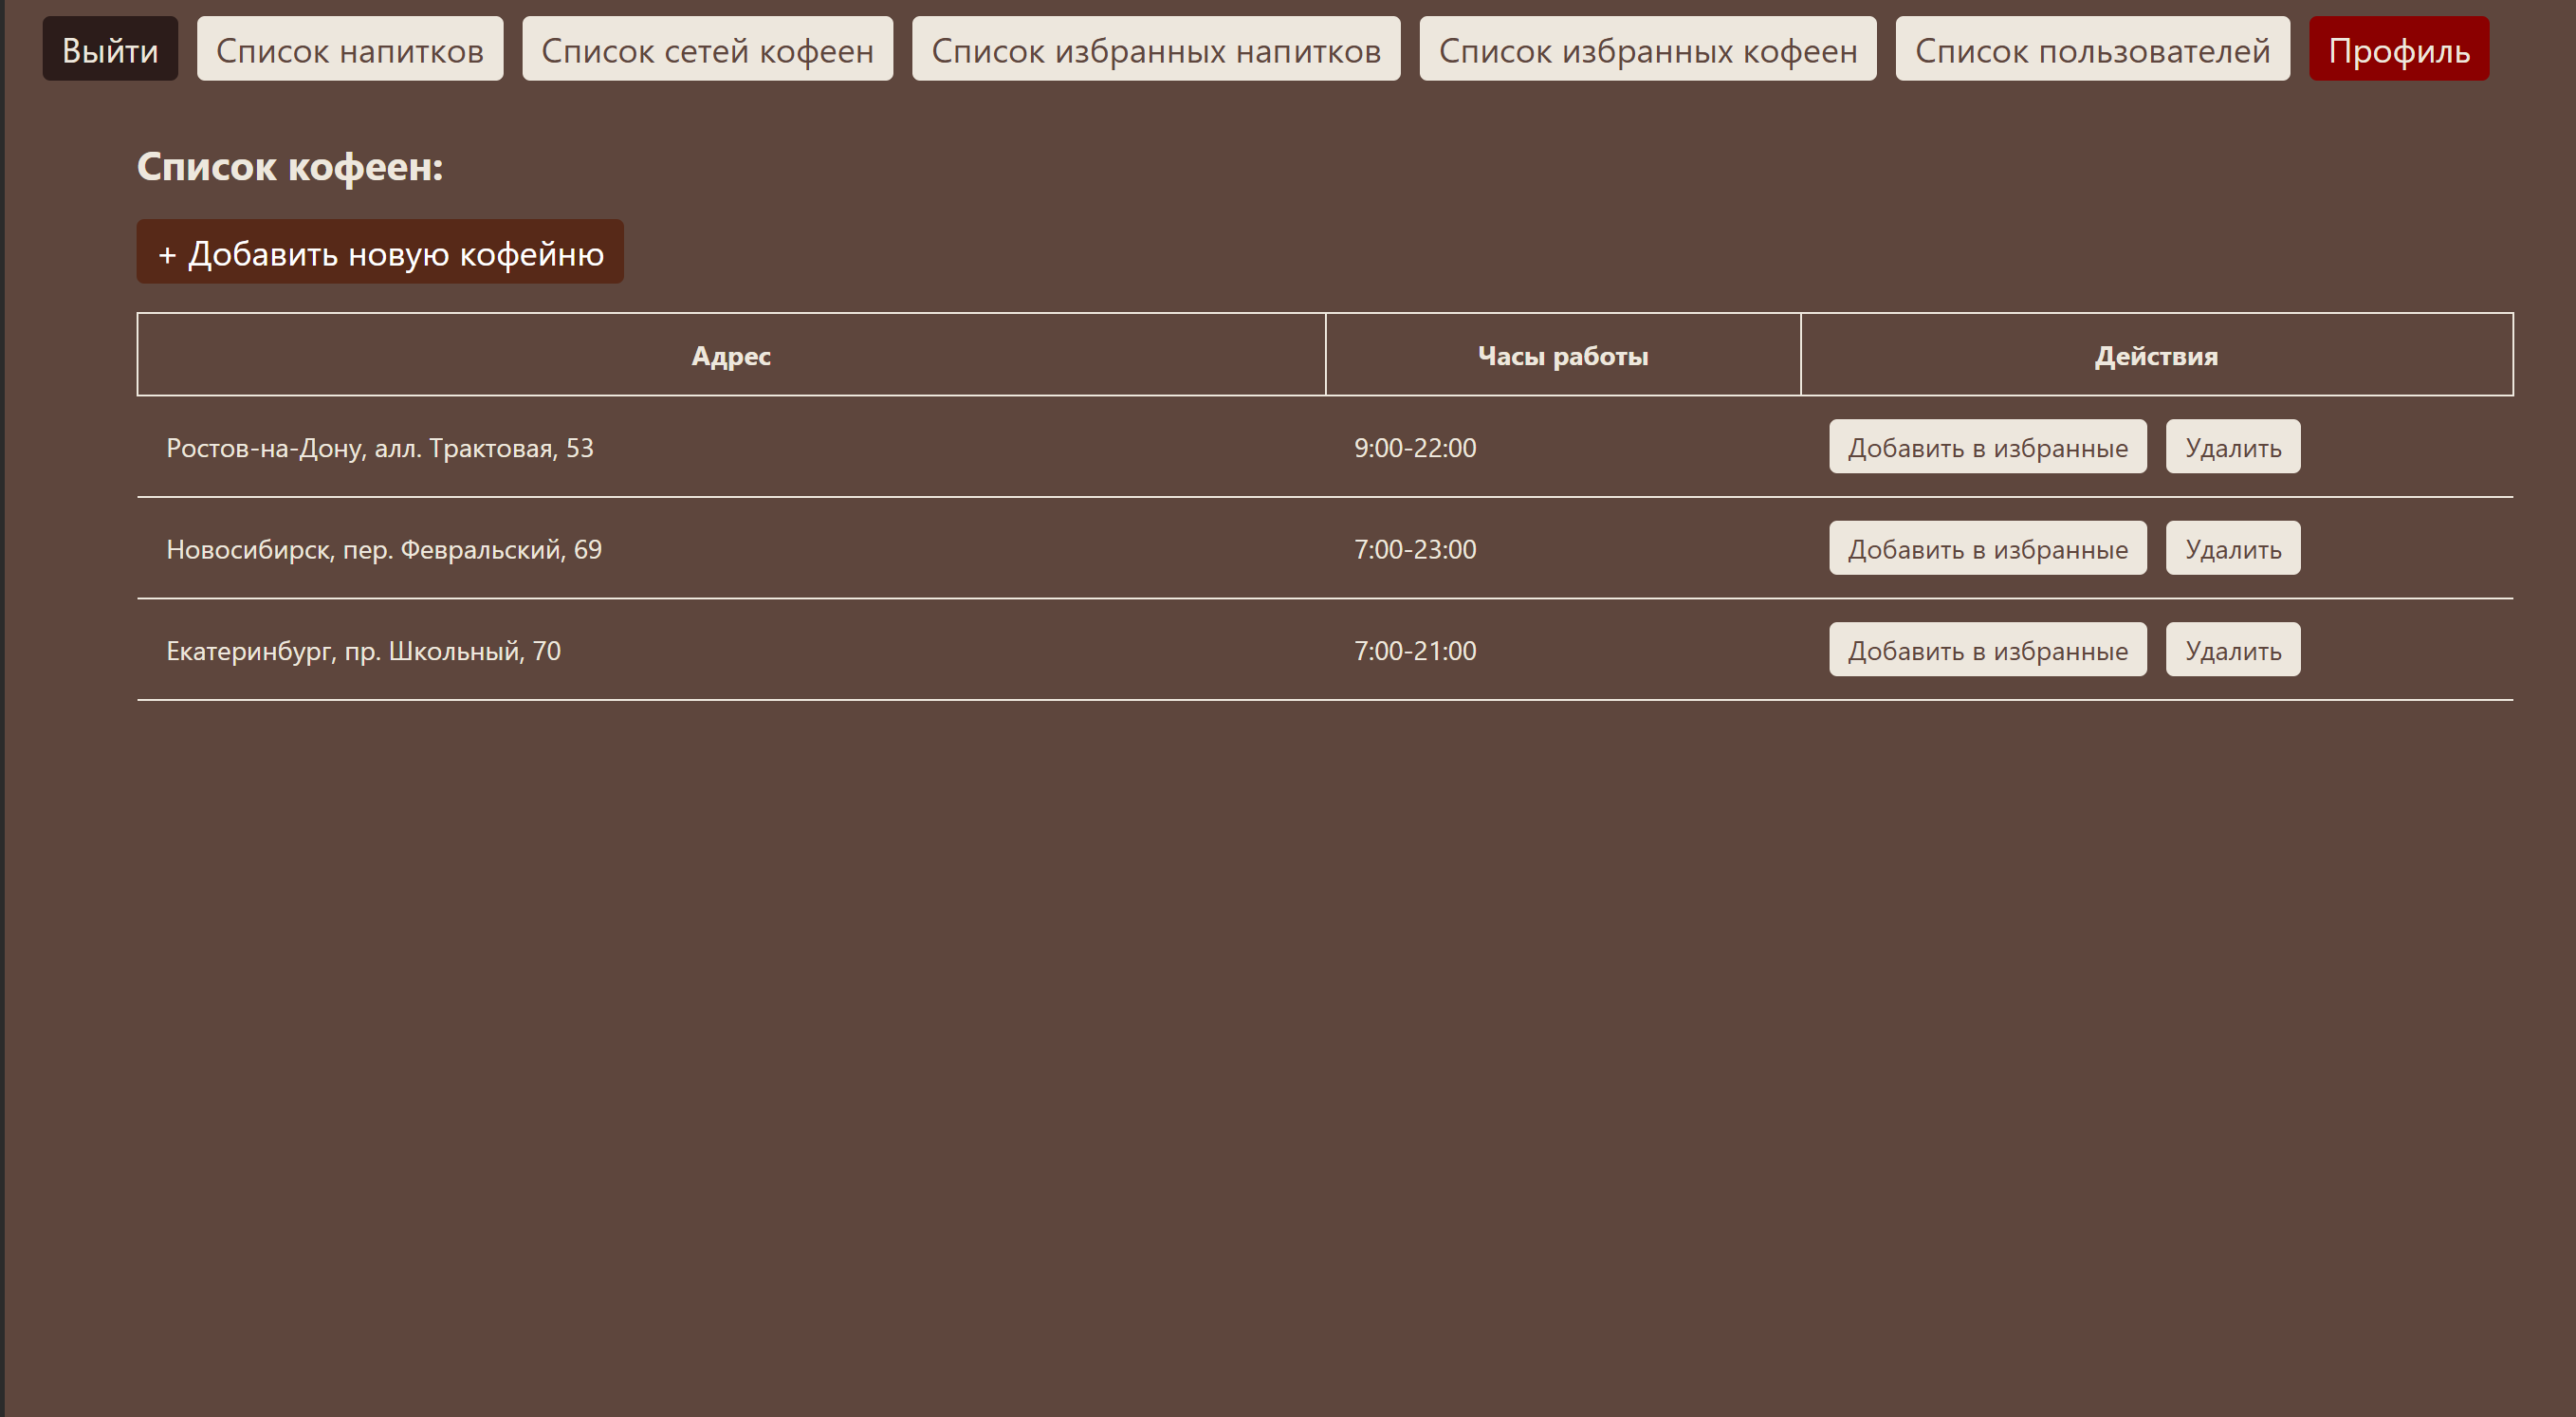
\includegraphics[width=1\linewidth]{img/interface/getcoffeeshops_admin.png}
	\caption{Страница с информацией о кофейнях конкретной сети (для обычных пользователей кнопки добавления и удаления кофеен недоступны)}
	\label{getcoffeeshops}
\end{figure}


\begin{figure}[H]
	\centering
	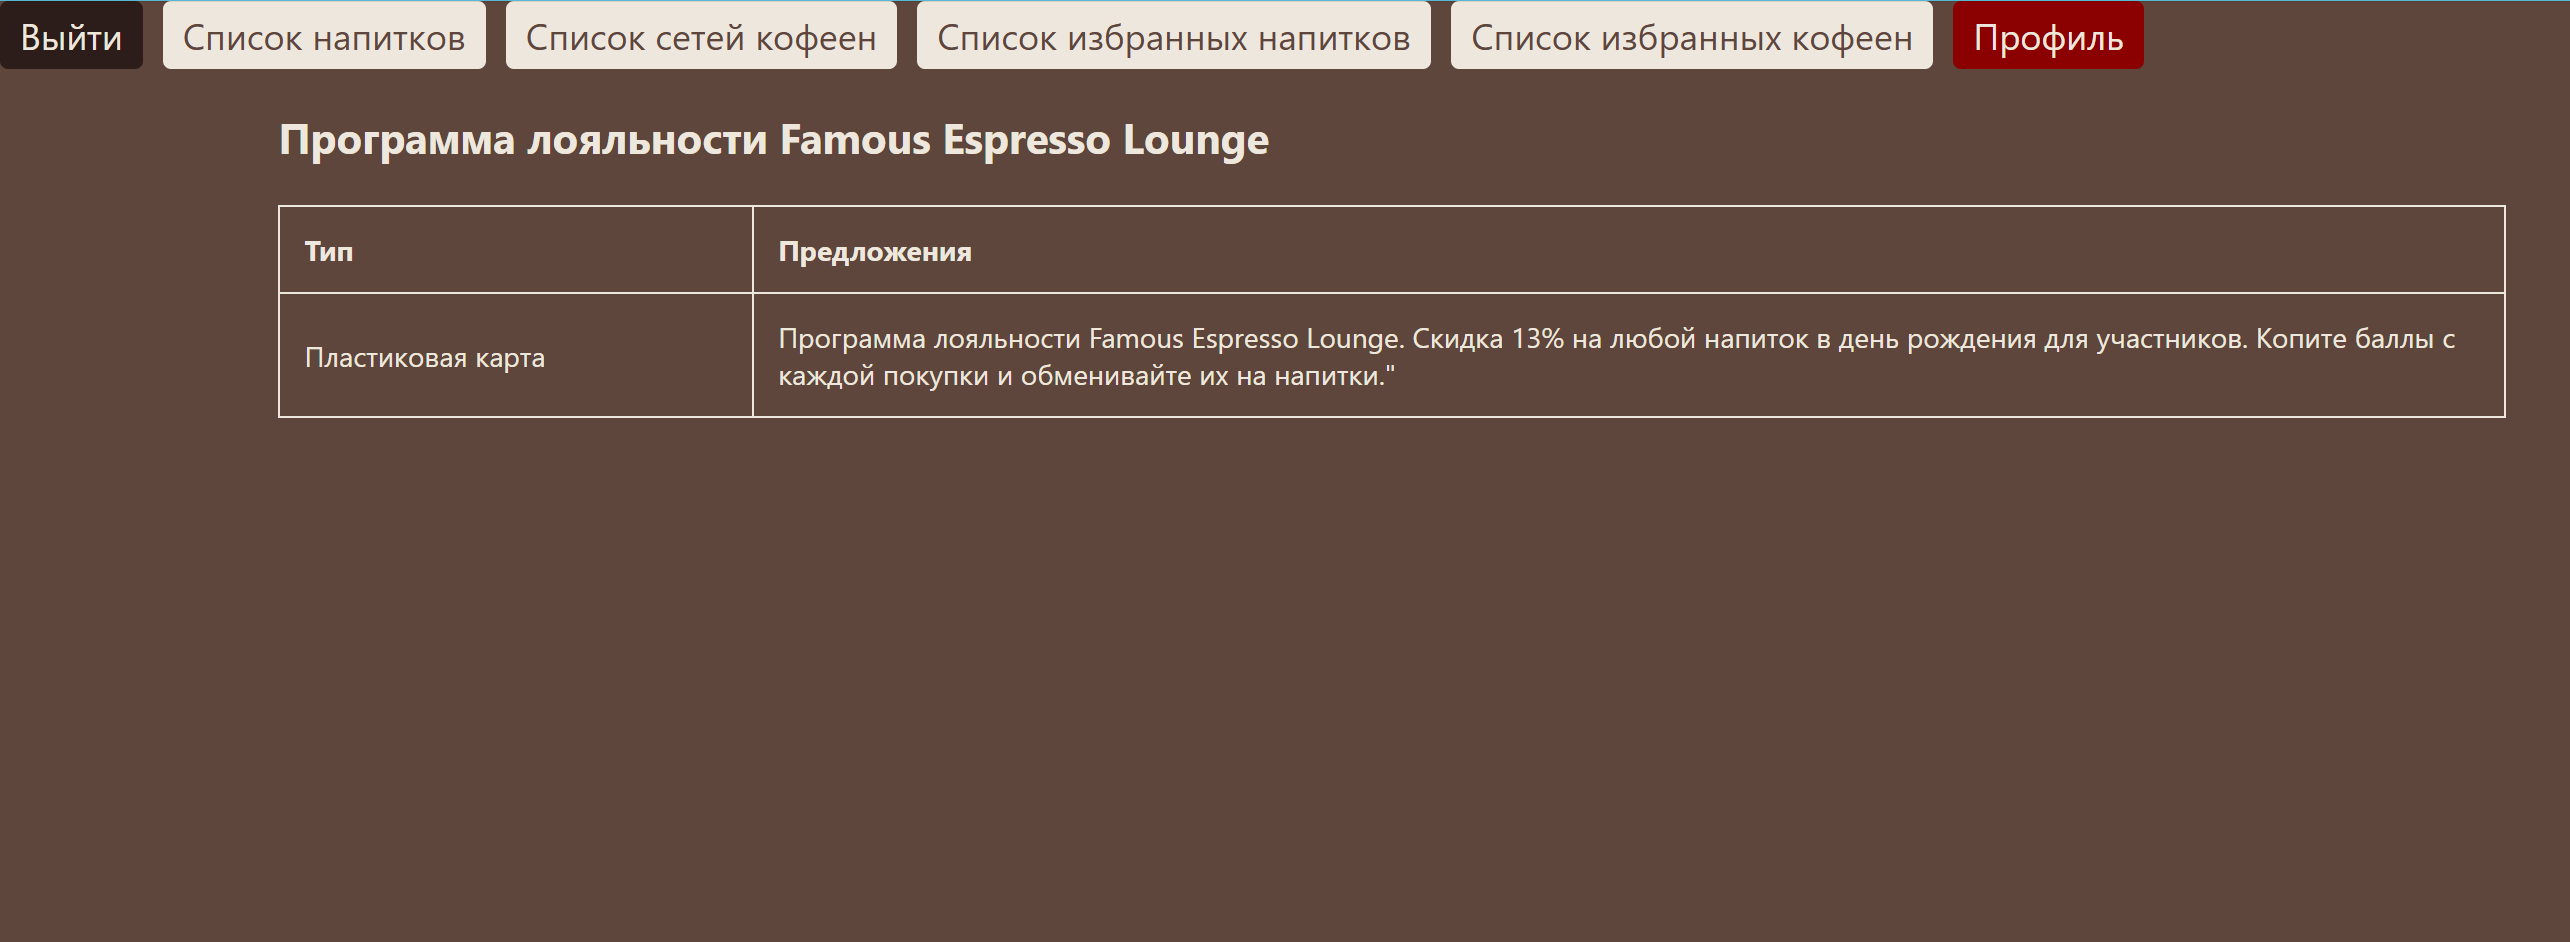
\includegraphics[width=1\linewidth]{img/interface/getlpbycompany.png}
	\caption{Страница с информацией о программе лояльности конкретной сети кофеен}
	\label{getlpbycompany}
\end{figure}

\begin{figure}[H]
	\centering
	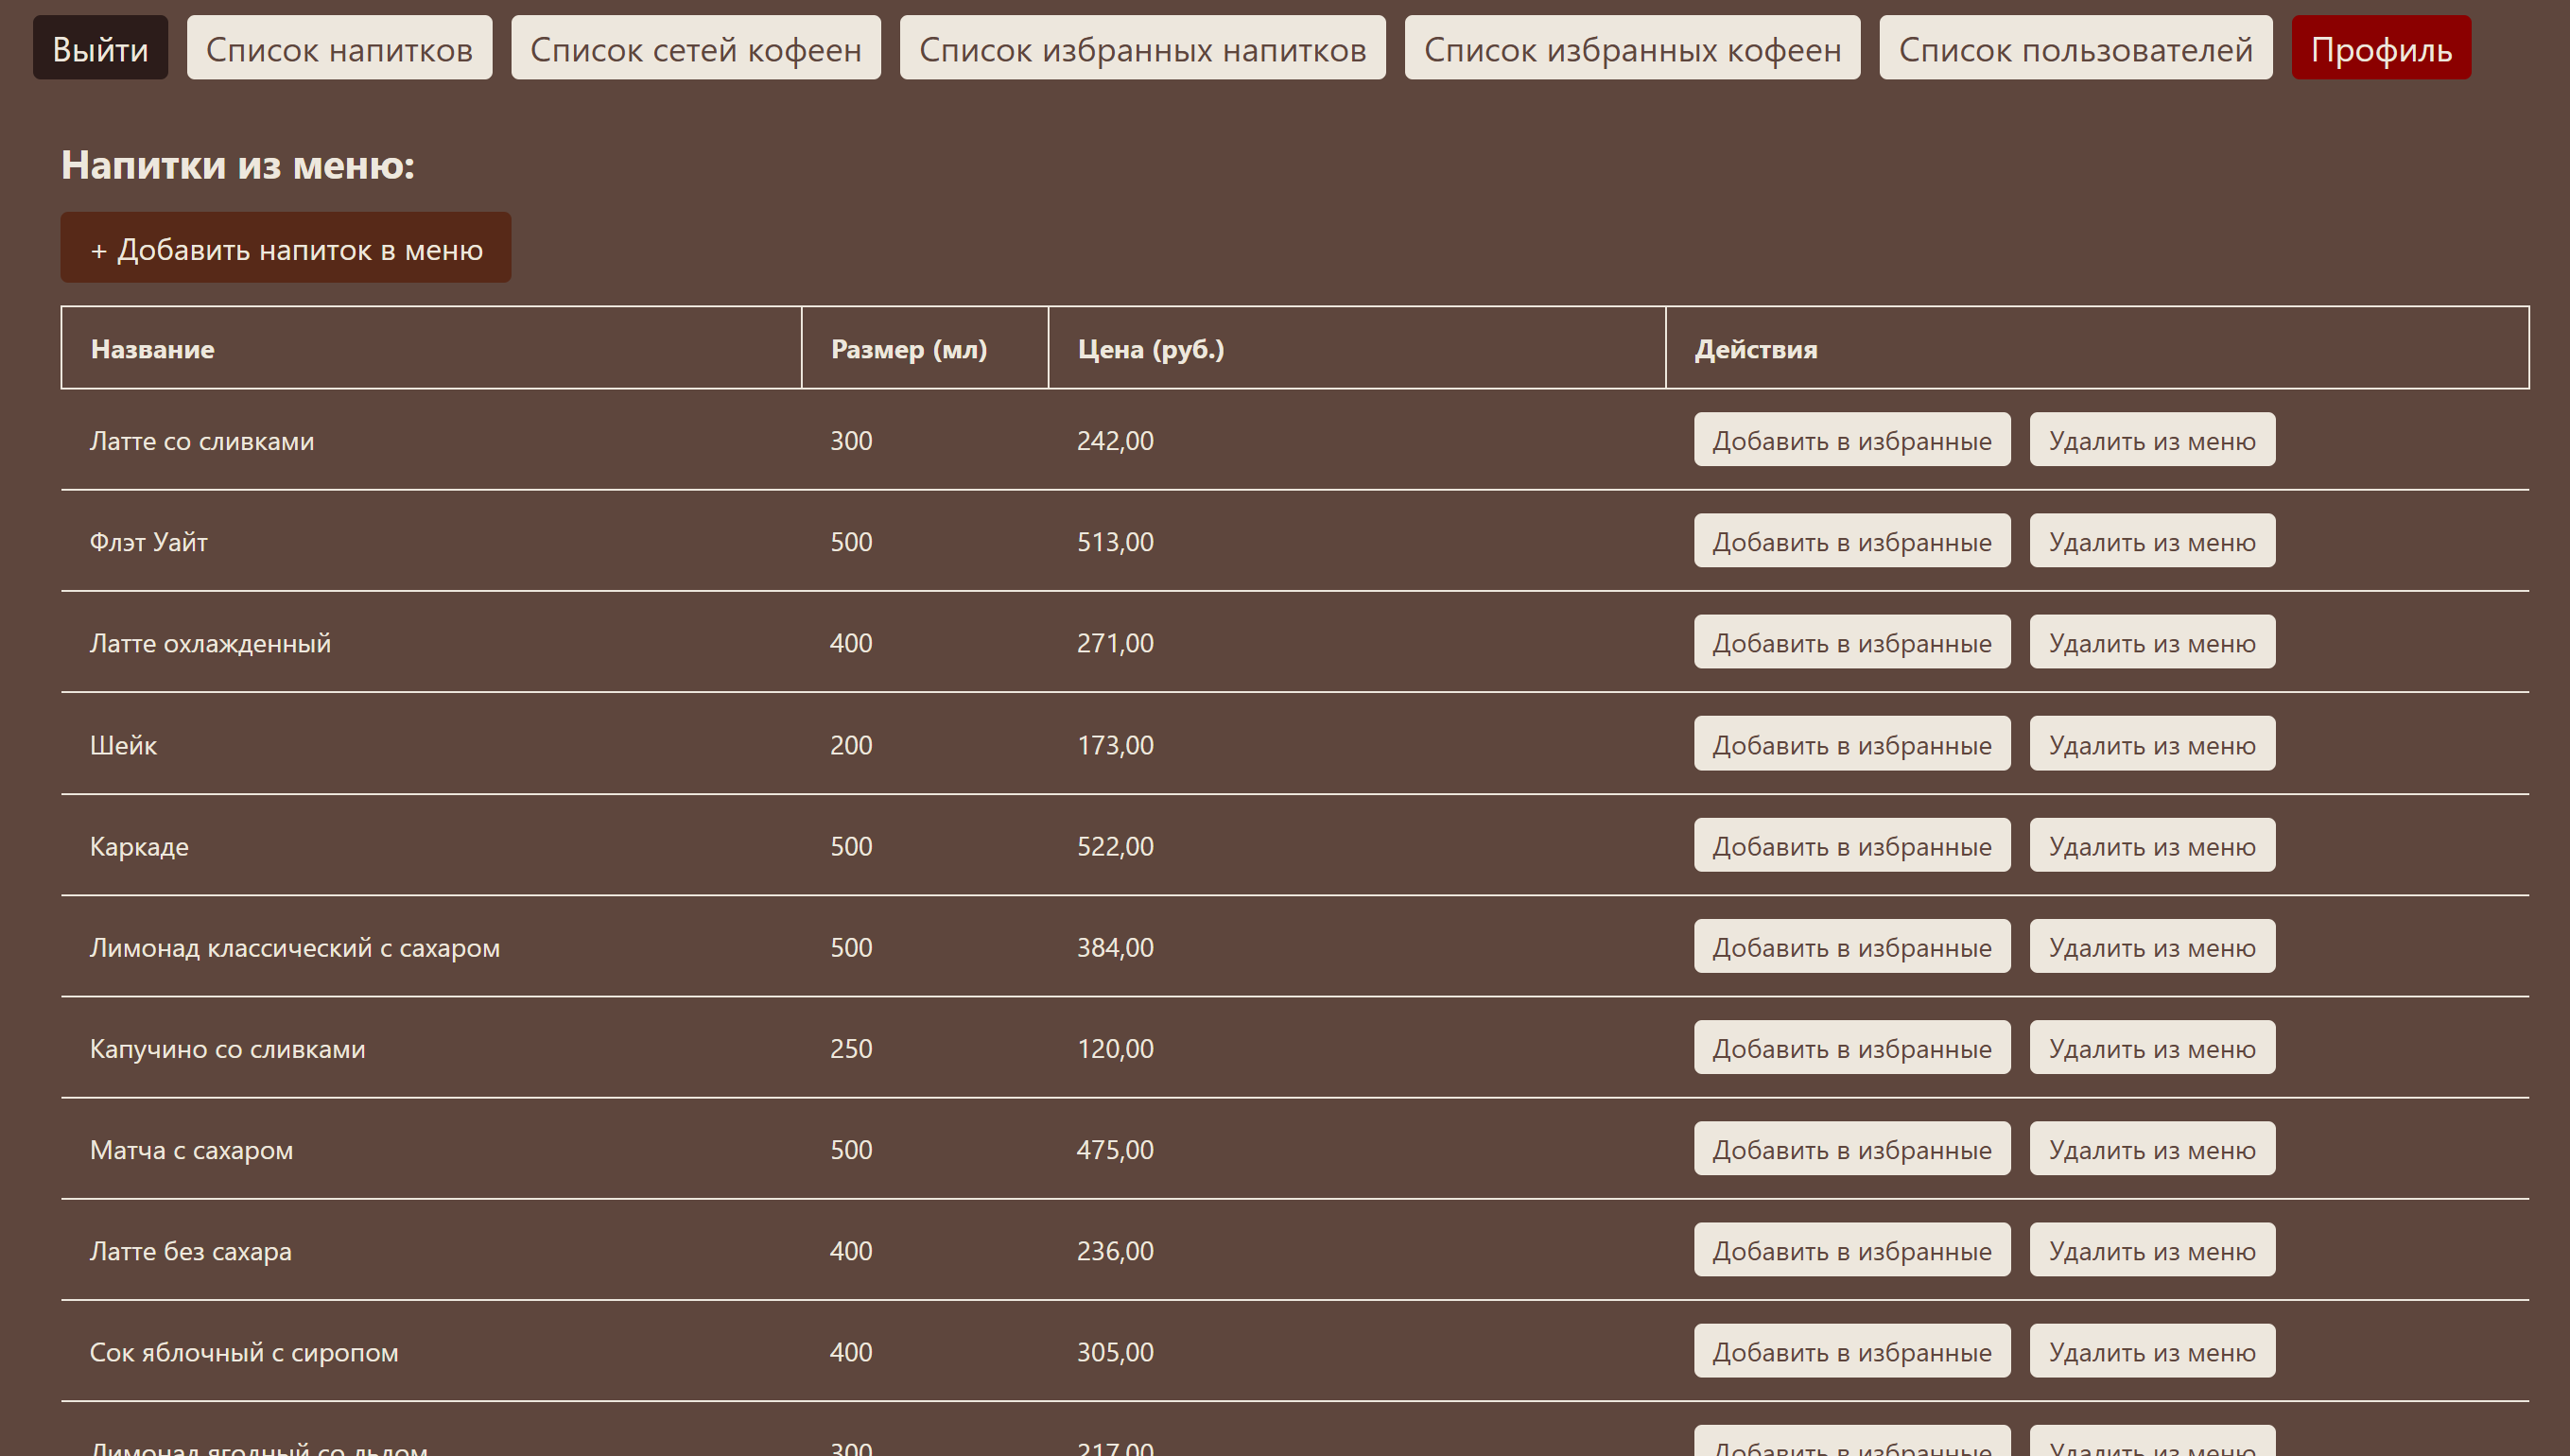
\includegraphics[width=1\linewidth]{img/interface/menu_admin.png}
	\caption{Страница с меню конкретной сети кофеен (для обычных пользователей кнопки добавления и удаления позиций меню недоступны)}
	\label{menu}
\end{figure}

\begin{figure}[H]
	\centering
	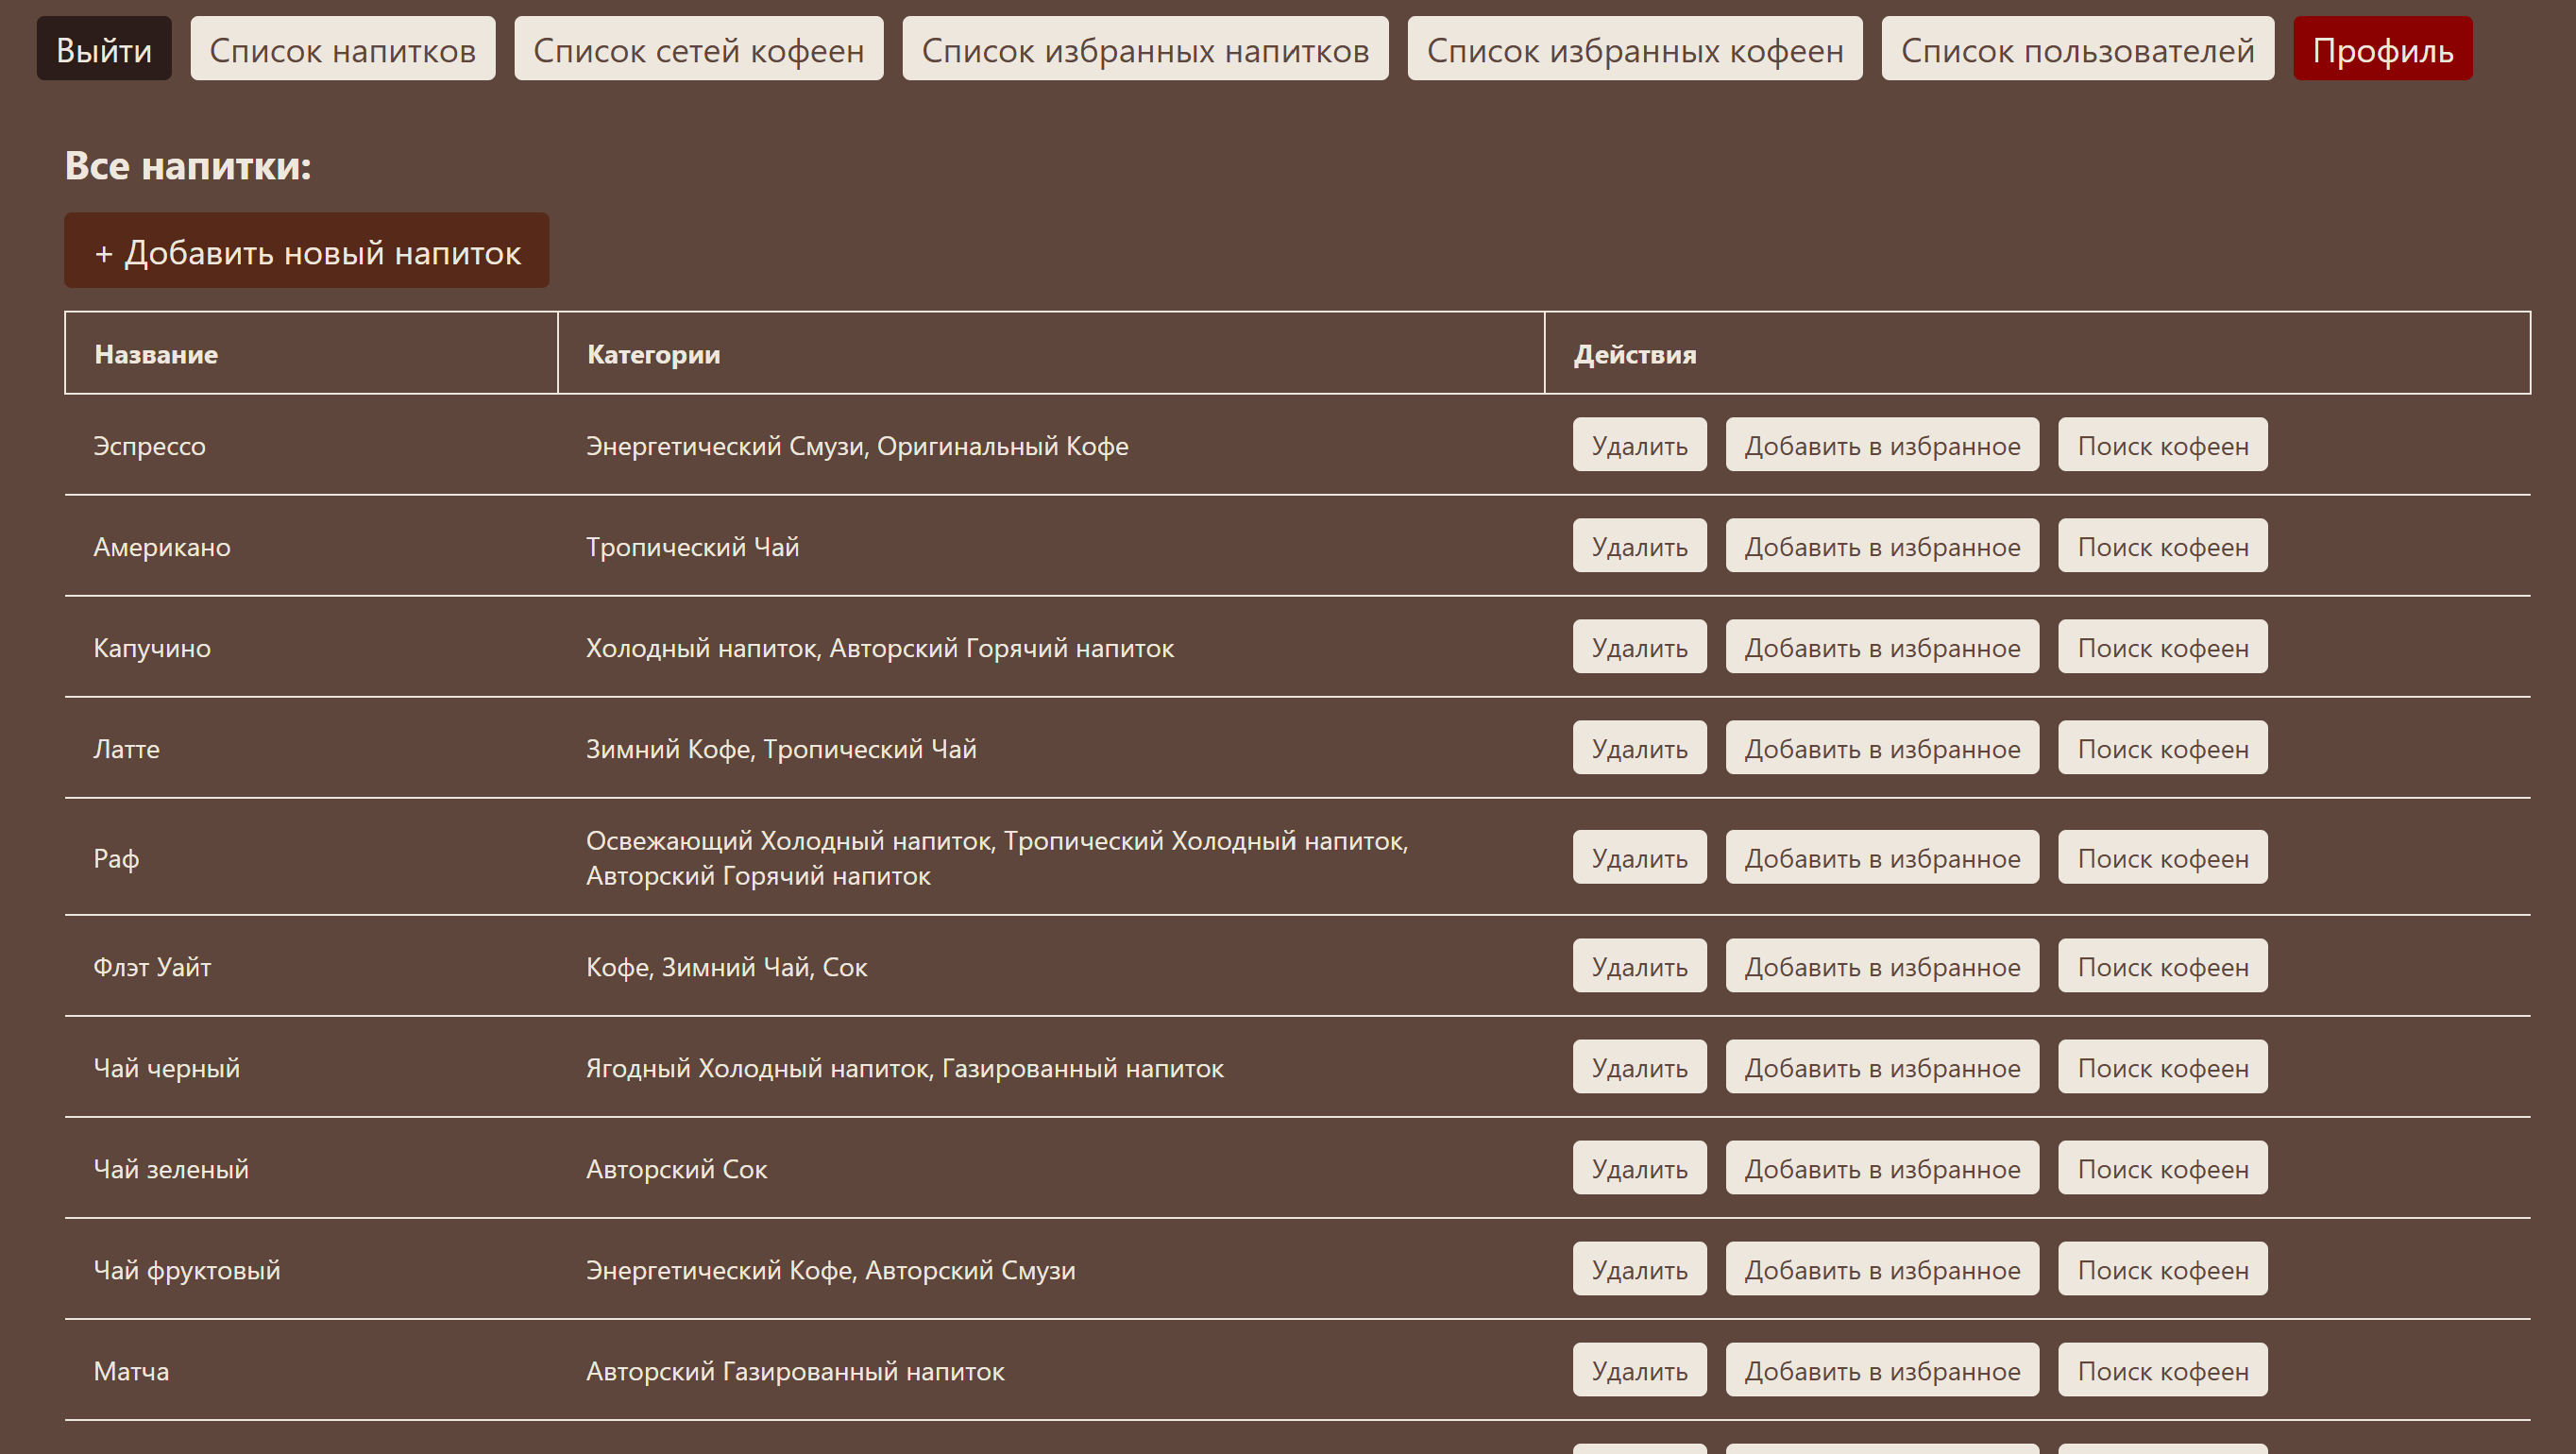
\includegraphics[width=1\linewidth]{img/interface/alldrinks_admin.png}
	\caption{Страница с всеми напитками, имеющимися в базе данных (для обычных пользователей кнопки добавления и удаления напитков недоступны)}
	\label{alldrinks}
\end{figure}

\begin{figure}[H]
	\centering
	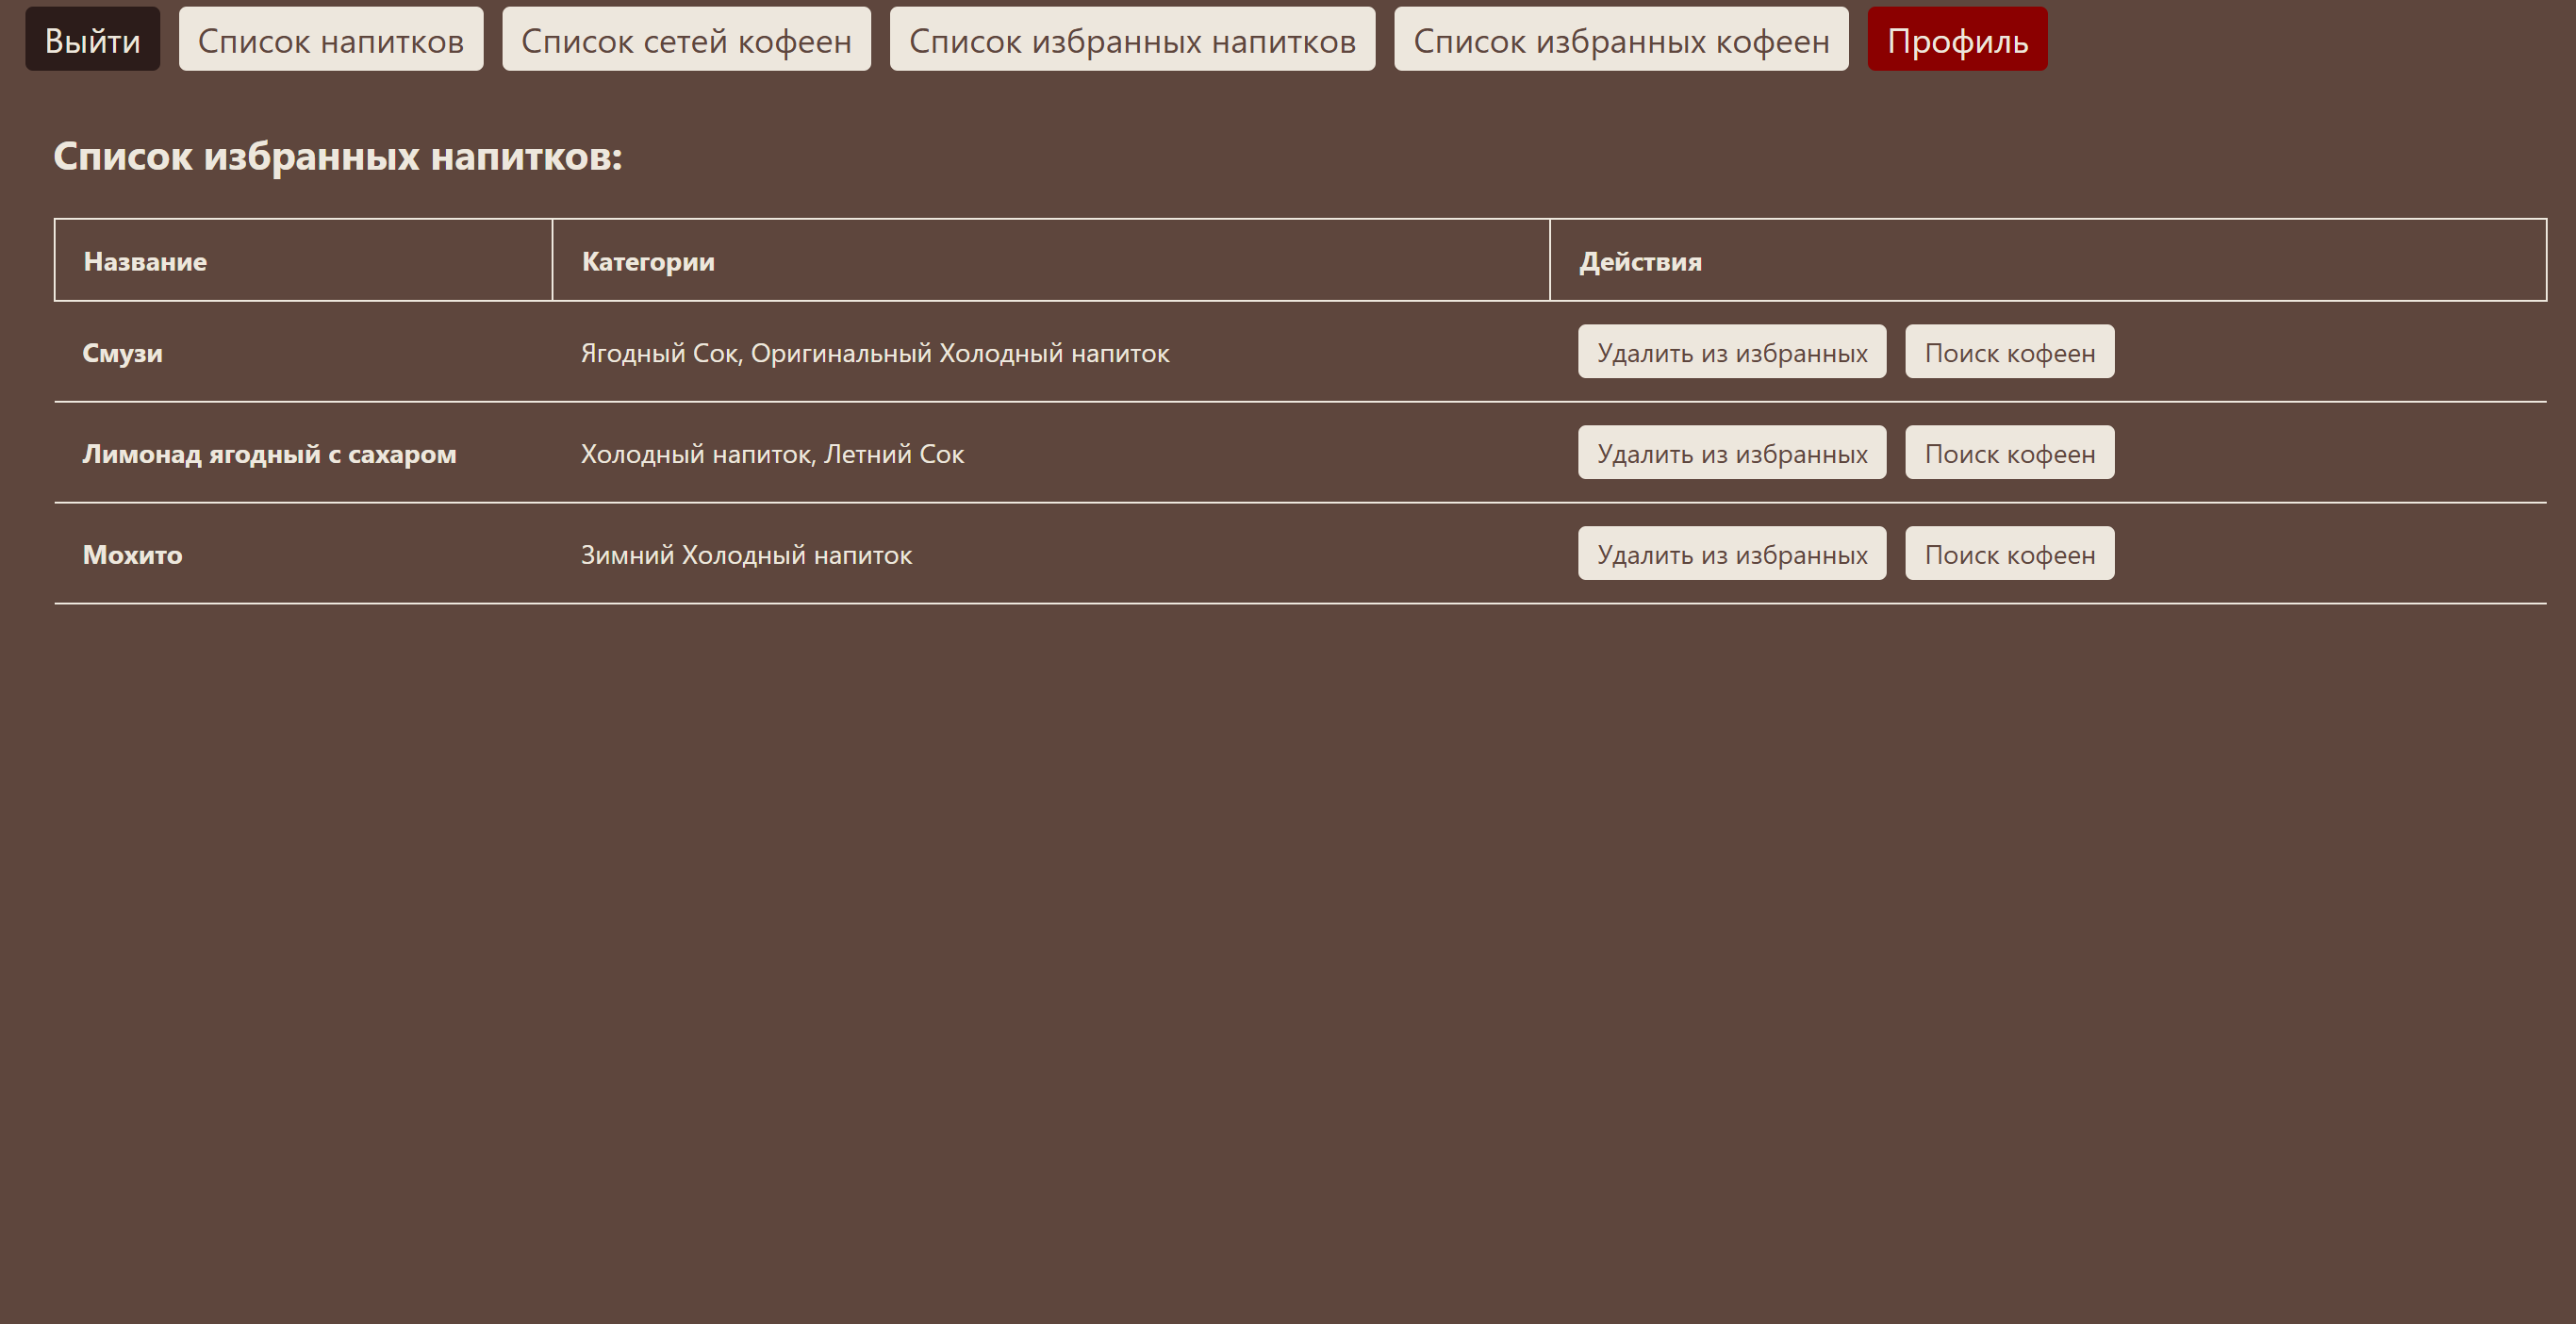
\includegraphics[width=1\linewidth]{img/interface/favdrinks.png}
	\caption{Страница с избранными напитками}
	\label{favdrinks}
\end{figure}

\begin{figure}[H]
	\centering
	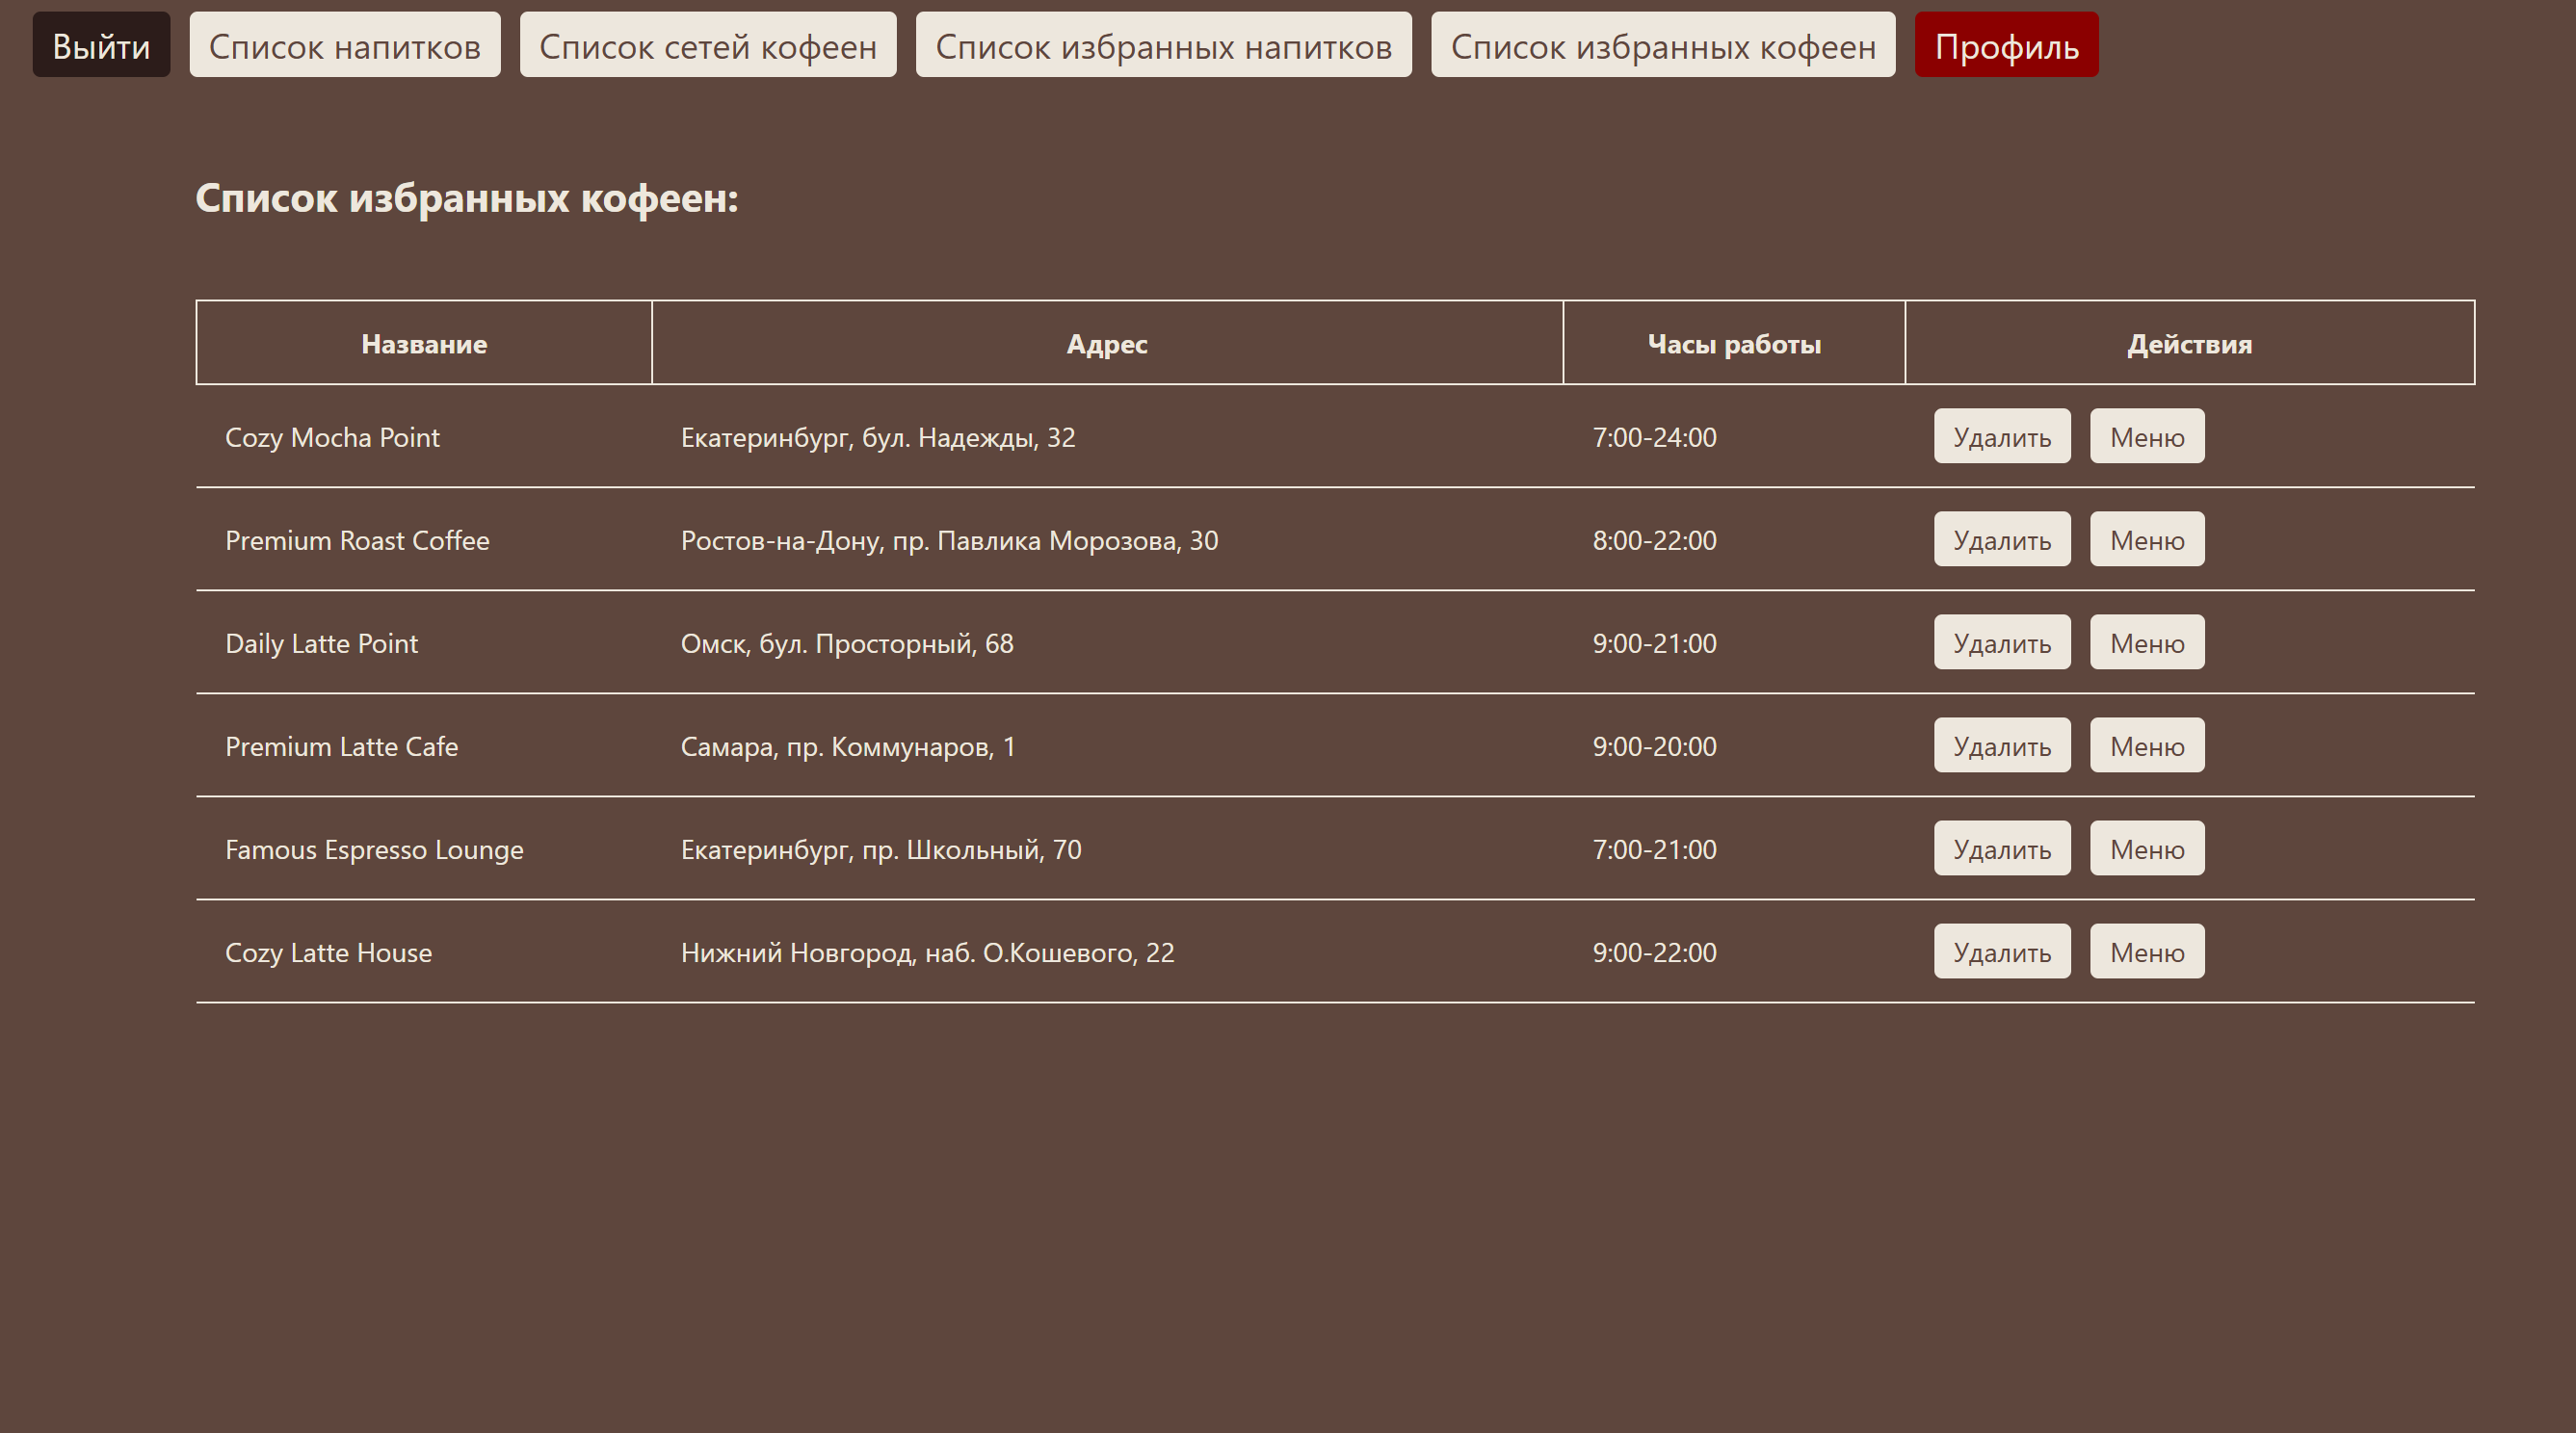
\includegraphics[width=1\linewidth]{img/interface/favcs.png}
	\caption{Страница с избранными кофейнями}
	\label{favcs}
\end{figure}

\begin{figure}[H]
	\centering
	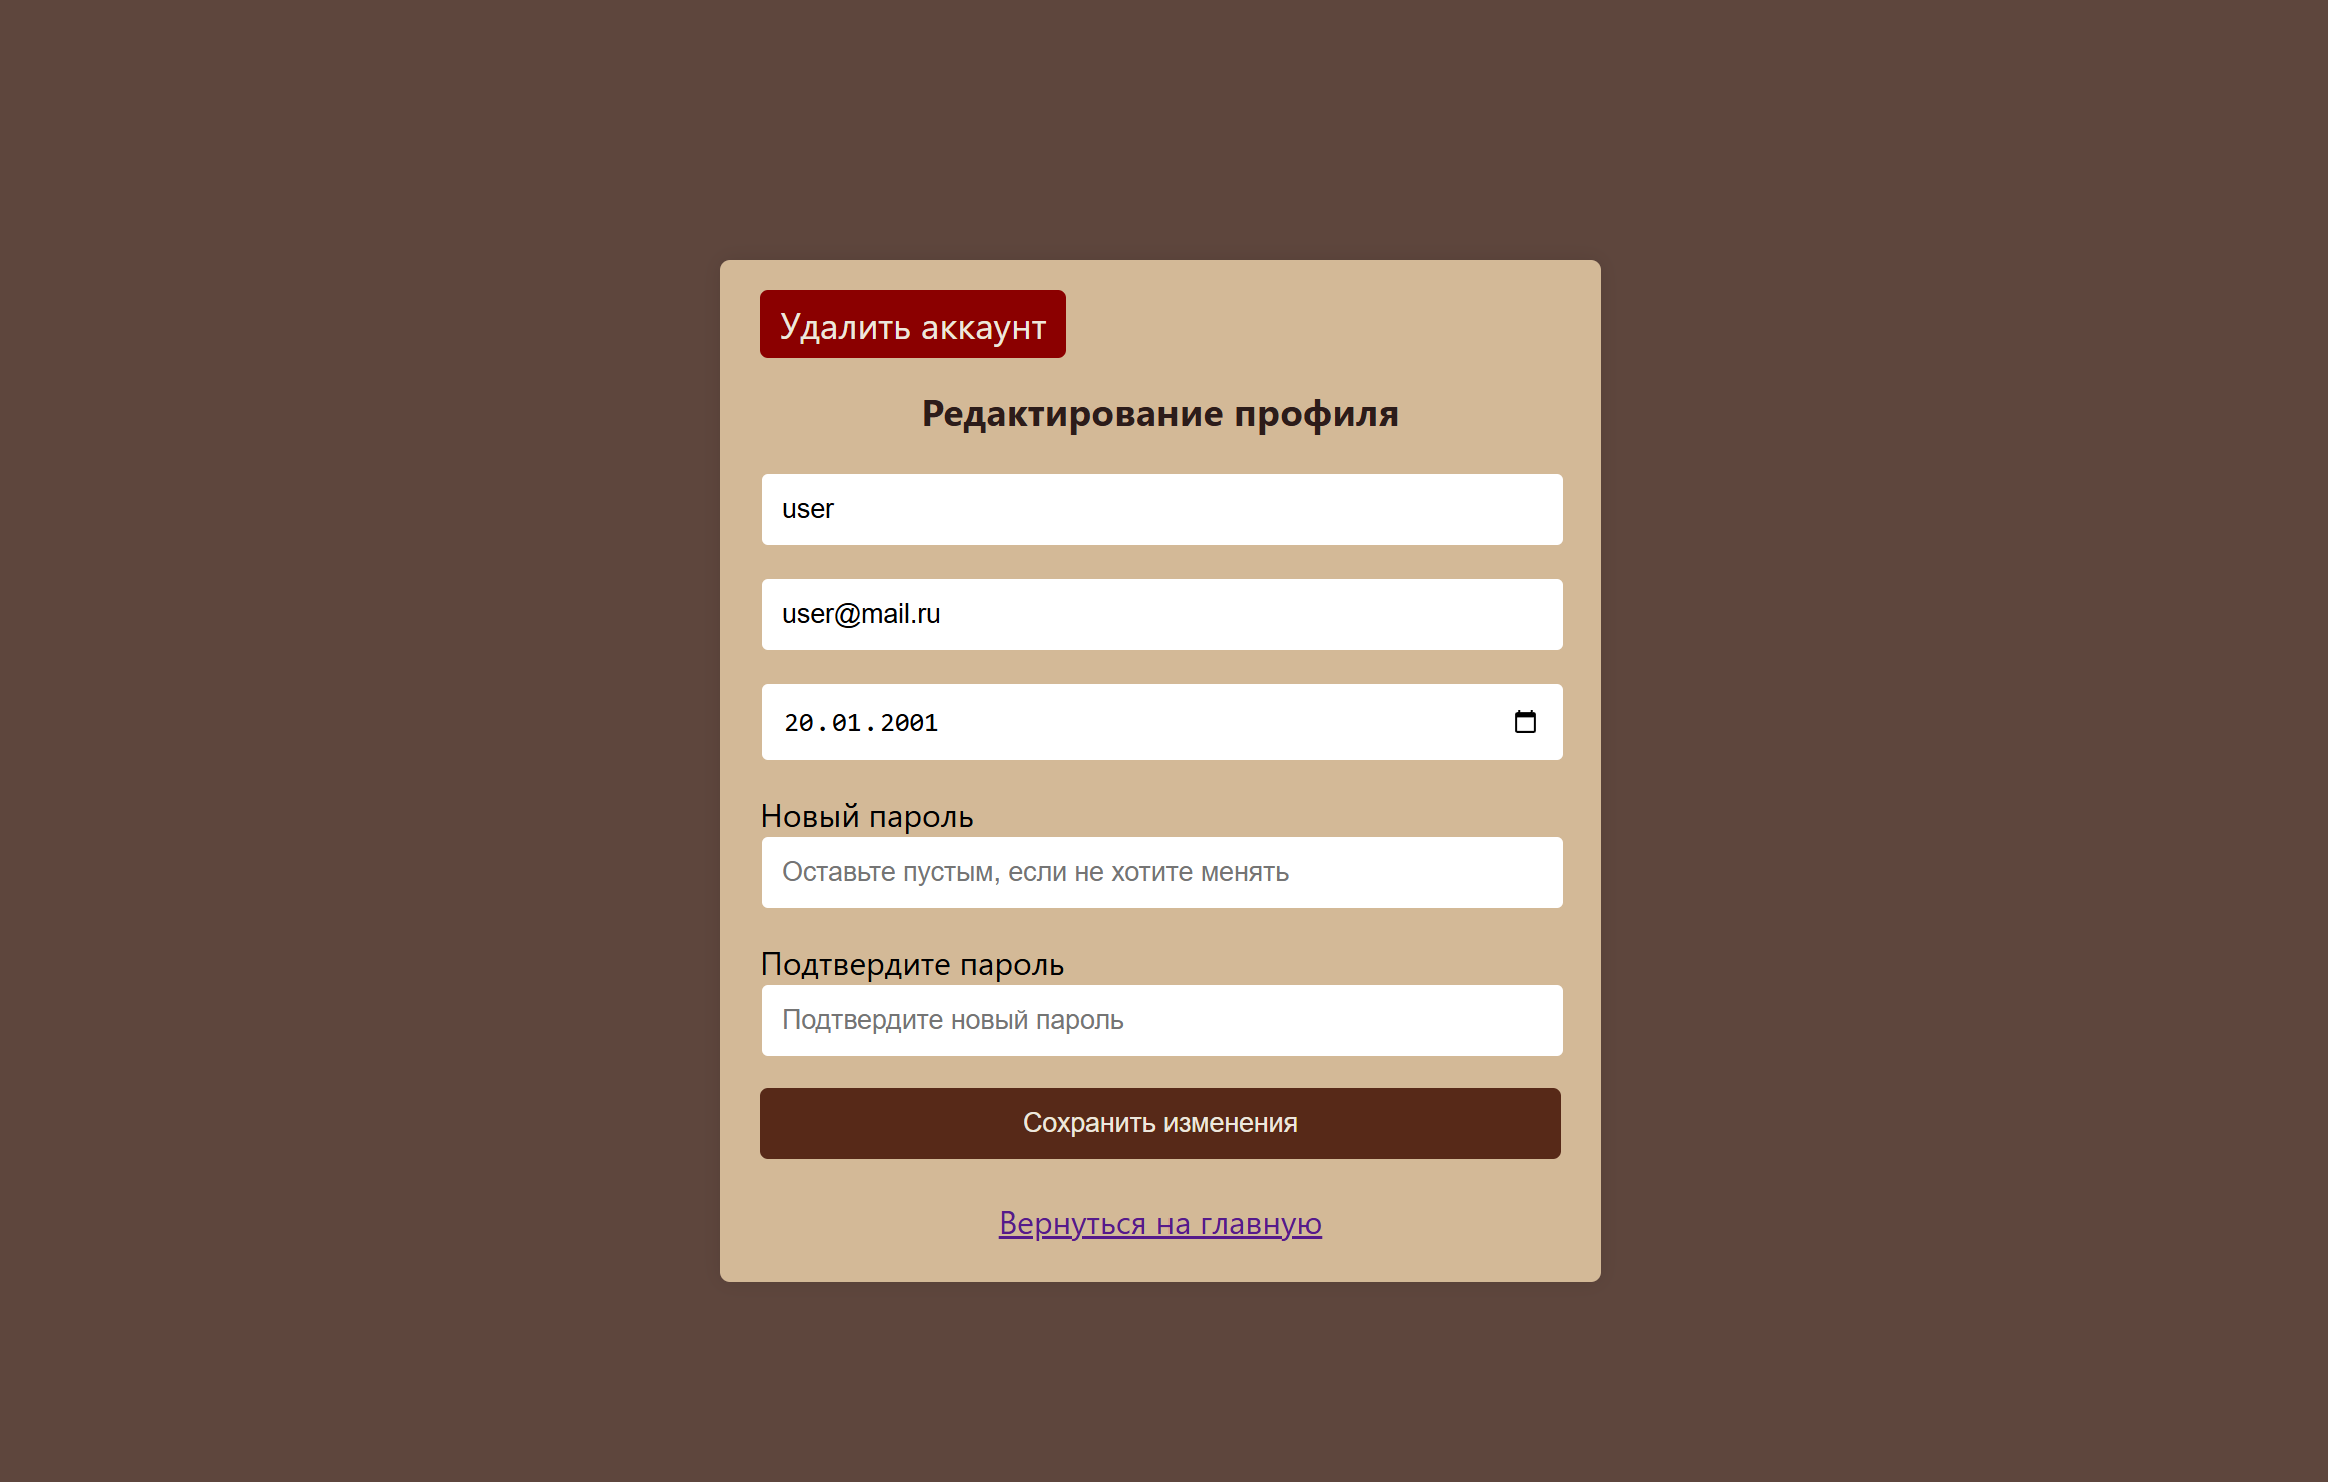
\includegraphics[width=1\linewidth]{img/interface/editprofile.png}
	\caption{Страница с изменением данных профиля}
	\label{editprofile}
\end{figure}

\begin{figure}[H]
	\centering
	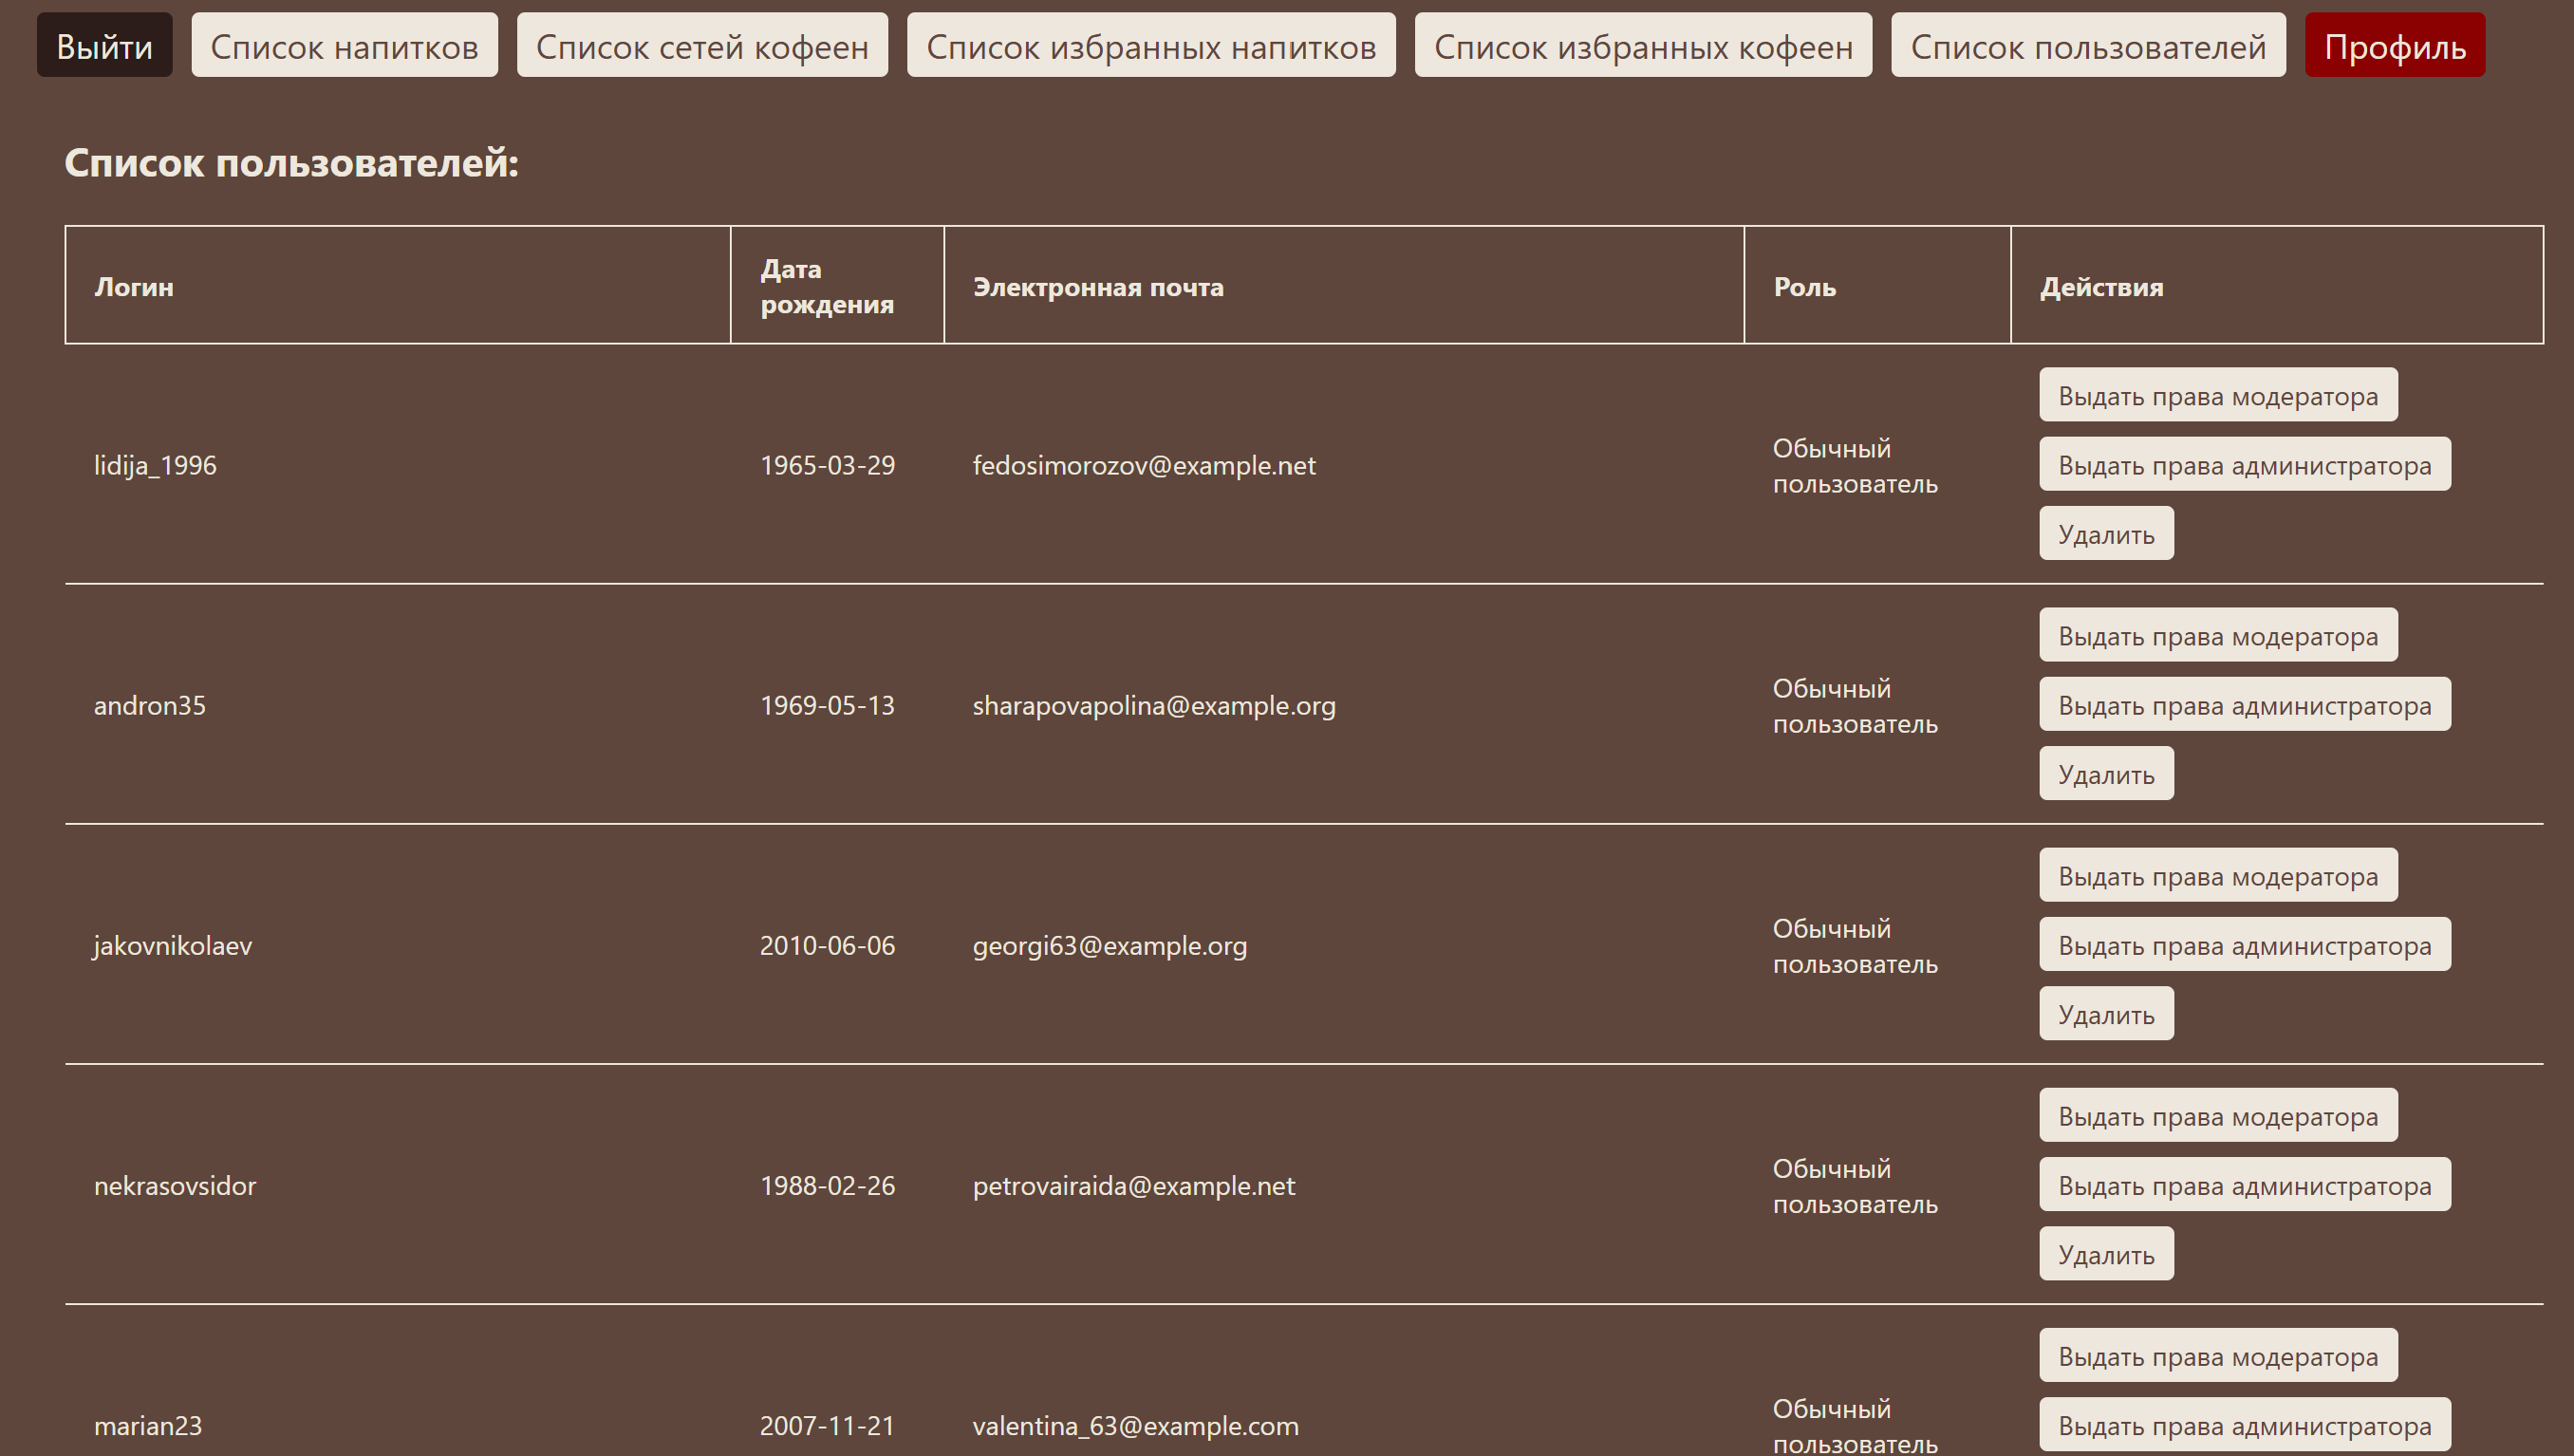
\includegraphics[width=1\linewidth]{img/interface/users.png}
	\caption{Страница с информацией о пользователях (доступна только администраторам)}
	\label{users}
\end{figure}


\section*{Вывод}
В данной части было проведено сравнение СУБД, в результате чего выбрана PostgreSQL. Также были разработаны описанные ранее объекты базы данных и приложение для доступа к ней.
